% !TeX spellcheck = en_GB
% !TeX encoding = UTF-8
% !TeX program = xelatex
% TODO Change language to en_GB (recommended) or en_US for English documents
\documentclass[11pt,a4paper,oneside]{report}             % Single-side
%\documentclass[11pt,a4paper,twoside,openright]{report}  % Duplex

% thanks to http://tex.stackexchange.com/a/47579/71109
\usepackage{ifxetex}
\usepackage{ifluatex}
\newif\ifxetexorluatex % a new conditional starts as false
\ifnum 0\ifxetex 1\fi\ifluatex 1\fi>0
   \xetexorluatextrue
\fi

\ifxetexorluatex
  \usepackage{fontspec}
\else
  \usepackage[T1]{fontenc}
  \usepackage[utf8]{inputenc}
  \usepackage[lighttt]{lmodern}
\fi

\usepackage[english,magyar]{babel} % Alapértelmezés szerint utoljára definiált nyelv lesz aktív, de később külön beállítjuk az aktív nyelvet.

%\usepackage{cmap}
\usepackage{amsfonts,amsmath,amssymb} % Mathematical symbols.
%\usepackage[ruled,boxed,resetcount,linesnumbered]{algorithm2e} % For pseudocodes. % beware: this is not compatible with LuaLaTeX, see http://tex.stackexchange.com/questions/34814/lualatex-and-algorithm2e
\usepackage{booktabs} % For publication quality tables for LaTeX
\usepackage{graphicx}

%\usepackage{fancyhdr}
%\usepackage{lastpage}

\usepackage{anysize}
%\usepackage{sectsty}
\usepackage{setspace} % For setting line spacing

\usepackage[unicode,colorlinks=true,linkcolor=blue]{hyperref} % For hyperlinks in the generated document.

\usepackage{xcolor}
\usepackage{listings} % For source code snippets.

\usepackage[amsmath,thmmarks]{ntheorem} % Theorem-like environments.

\usepackage[hang]{caption}

\singlespacing

\newcommand{\selecthungarian}{
	\selectlanguage{magyar}
	\setlength{\parindent}{2em}
	\setlength{\parskip}{0em}
	\frenchspacing
}

\newcommand{\selectenglish}{
	\selectlanguage{english}
	\setlength{\parindent}{0em}
	\setlength{\parskip}{0.5em}
	\nonfrenchspacing
	\renewcommand{\figureautorefname}{Figure}
	\renewcommand{\tableautorefname}{Table}
	\renewcommand{\partautorefname}{Part}
	\renewcommand{\chapterautorefname}{Chapter}
	\renewcommand{\sectionautorefname}{Section}
	\renewcommand{\subsectionautorefname}{Section}
	\renewcommand{\subsubsectionautorefname}{Section}
}

\usepackage[numbers]{natbib}
\usepackage{xspace}


%TODO Set the main variables
\newcommand{\vikszerzoVezeteknev}{Péter}
\newcommand{\vikszerzoKeresztnev}{István}

\newcommand{\vikkonzulensAMegszolitas}{dr.~}
\newcommand{\vikkonzulensAVezeteknev}{Kiss}
\newcommand{\vikkonzulensAKeresztnev}{Bálint}

\newcommand{\vikkonzulensBMegszolitas}{}
\newcommand{\vikkonzulensBVezeteknev}{Nemes}
\newcommand{\vikkonzulensBKeresztnev}{Ádám Gyula}

\newcommand{\vikcim}{Comparison of convolution and transformer-based image processing neural networks} % Cím
\newcommand{\viktanszek}{\bmeiit} % Tanszék
\newcommand{\vikdoktipus}{\bsc} % Dokumentum típusa (\bsc vagy \msc)
\newcommand{\vikmunkatipusat}{szakdolgozatot} % a "hallgató nyilatkozat" részhez: szakdolgozatot vagy diplomatervet

%--------------------------------------------------------------------------------------
% TDK-specifikus változók
%--------------------------------------------------------------------------------------
\newcommand{\tdkszerzoB}{Második Szerző} % Második szerző neve; hagyd üresen, ha egyedül írtad a TDK-t.
\newcommand{\tdkev}{2014} % A dolgozat írásának éve (pl. "2014") (Ez OTDK-nál eltérhet az aktuális évtől.)

% További adatok az OTDK címlaphoz (BME-s TDK-hoz nem kell kitölteni)
\newcommand{\tdkevfolyamA}{IV} % Első szerző évfolyama, római számmal (pl. IV).
\newcommand{\tdkevfolyamB}{III} % Második szerző évfolyama, római számmal (pl. III).
\newcommand{\tdkkonzulensbeosztasA}{egyetemi tanár} % Első konzulens beosztása (pl. egyetemi docens)
\newcommand{\tdkkonzulensbeosztasB}{doktorandusz} % Második konzulens beosztása (pl. egyetemi docens)

\newcommand{\szerzoMeta}{\vikszerzoVezeteknev{} \vikszerzoKeresztnev} % egy szerző esetén
%\newcommand{\szerzoMeta}{\vikszerzoVezeteknev{} \vikszerzoKeresztnev, \tdkszerzoB} % két szerző esetén

%TODO Language configuration -- choose one
% Beállítások magyar nyelvű dolgozathoz
%%--------------------------------------------------------------------------------------
% Elnevezések
%--------------------------------------------------------------------------------------
\newcommand{\bme}{Budapesti Műszaki és Gazdaságtudományi Egyetem}
\newcommand{\vik}{Villamosmérnöki és Informatikai Kar}

\newcommand{\bmemit}{Méréstechnika és Információs Rendszerek Tanszék}

\newcommand{\keszitette}{Készítette}
\newcommand{\konzulens}{Konzulens}

\newcommand{\bsc}{Szakdolgozat}
\newcommand{\msc}{Diplomaterv}
\newcommand{\tdk}{TDK dolgozat}
\newcommand{\bsconlab}{BSc Önálló laboratórium}
\newcommand{\msconlabi}{MSc Önálló laboratórium 1.}
\newcommand{\msconlabii}{MSc Önálló laboratórium 2.}

\newcommand{\pelda}{Példa}
\newcommand{\definicio}{Definíció}
\newcommand{\tetel}{Tétel}

\newcommand{\bevezetes}{Bevezetés}
\newcommand{\koszonetnyilvanitas}{Köszönetnyilvánítás}
\newcommand{\fuggelek}{Függelék}

% Opcionálisan átnevezhető címek
%\addto\captionsmagyar{%
%\renewcommand{\listfigurename}{Saját ábrajegyzék cím}
%\renewcommand{\listtablename}{Saját táblázatjegyzék cím}
%\renewcommand{\bibname}{Saját irodalomjegyzék név}
%}

\newcommand{\szerzo}{\vikszerzoVezeteknev{} \vikszerzoKeresztnev}
\newcommand{\vikkonzulensA}{\vikkonzulensAMegszolitas\vikkonzulensAVezeteknev{} \vikkonzulensAKeresztnev}
\newcommand{\vikkonzulensB}{\vikkonzulensBMegszolitas\vikkonzulensBVezeteknev{} \vikkonzulensBKeresztnev}
\newcommand{\vikkonzulensC}{\vikkonzulensCMegszolitas\vikkonzulensCVezeteknev{} \vikkonzulensCKeresztnev}

\newcommand{\selectthesislanguage}{\selecthungarian}

\bibliographystyle{huplain}

\def\lstlistingname{lista}

\newcommand{\appendixnumber}{6}  % a fofejezet-szamlalo az angol ABC 6. betuje (F) lesz

% Settings for English documents
%--------------------------------------------------------------------------------------
% Elnevezések
%--------------------------------------------------------------------------------------
\newcommand{\bme}{Budapest University of Technology and Economics}
\newcommand{\vik}{Faculty of Electrical Engineering and Informatics}

\newcommand{\bmeiit}{Department of Control Engineering and Information Technology}

\newcommand{\keszitette}{Author}
\newcommand{\konzulens}{Advisor}

\newcommand{\bsc}{Bachelor's Thesis}
\newcommand{\msc}{Master's Thesis}
\newcommand{\tdk}{Scientific Students' Association Report}
\newcommand{\bsconlab}{BSc Project Laboratory}
\newcommand{\msconlabi}{MSc Project Laboratory 1}
\newcommand{\msconlabii}{MSc Project Laboratory 2}

\newcommand{\pelda}{Example}
\newcommand{\definicio}{Definition}
\newcommand{\tetel}{Theorem}

\newcommand{\bevezetes}{Introduction}
\newcommand{\koszonetnyilvanitas}{Acknowledgements}
\newcommand{\fuggelek}{Appendix}

% Optional custom titles
%\addto\captionsenglish{%
%\renewcommand*{\listfigurename}{Your list of figures title}
%\renewcommand*{\listtablename}{Your list of tables title}
%\renewcommand*{\bibname}{Your bibliography title}
%}

\newcommand{\szerzo}{\vikszerzoKeresztnev{} \vikszerzoVezeteknev}
\newcommand{\vikkonzulensA}{\vikkonzulensAMegszolitas\vikkonzulensAKeresztnev{} \vikkonzulensAVezeteknev}
\newcommand{\vikkonzulensB}{\vikkonzulensBMegszolitas\vikkonzulensBKeresztnev{} \vikkonzulensBVezeteknev}
\newcommand{\vikkonzulensC}{\vikkonzulensCMegszolitas\vikkonzulensCKeresztnev{} \vikkonzulensCVezeteknev}

\newcommand{\selectthesislanguage}{\selectenglish}

\bibliographystyle{plainnat}

\newcommand{\ie}{i.e.\@\xspace}
\newcommand{\Ie}{I.e.\@\xspace}
\newcommand{\eg}{e.g.\@\xspace}
\newcommand{\Eg}{E.g.\@\xspace}
\newcommand{\etal}{et al.\@\xspace}
\newcommand{\etc}{etc.\@\xspace}
\newcommand{\vs}{vs.\@\xspace}
\newcommand{\viz}{viz.\@\xspace} % videlicet
\newcommand{\cf}{cf.\@\xspace} % confer
\newcommand{\Cf}{Cf.\@\xspace}
\newcommand{\wrt}{w.r.t.\@\xspace} % with respect to
\newcommand{\approximately}{approx.\@\xspace}

\newcommand{\appendixnumber}{1}  % a fofejezet-szamlalo az angol ABC 1. betuje (A) lesz


%--------------------------------------------------------------------------------------
% Page layout setup
%--------------------------------------------------------------------------------------
% we need to redefine the pagestyle plain
% another possibility is to use the body of this command without \fancypagestyle
% and use \pagestyle{fancy} but in that case the special pages
% (like the ToC, the References, and the Chapter pages)remain in plane style

\pagestyle{plain}
\marginsize{35mm}{25mm}{15mm}{15mm}

\setcounter{tocdepth}{3}
%\sectionfont{\large\upshape\bfseries}
\setcounter{secnumdepth}{3}

\sloppy % Margón túllógó sorok tiltása.
\widowpenalty=10000 \clubpenalty=10000 %A fattyú- és árvasorok elkerülése
\def\hyph{-\penalty0\hskip0pt\relax} % Kötőjeles szavak elválasztásának engedélyezése


%--------------------------------------------------------------------------------------
% Setup hyperref package
%--------------------------------------------------------------------------------------
\hypersetup{
    % bookmarks=true,            % show bookmarks bar?
    unicode=true,              % non-Latin characters in Acrobat's bookmarks
    pdftitle={\vikcim},        % title
    pdfauthor={\szerzoMeta},    % author
    pdfsubject={\vikdoktipus}, % subject of the document
    pdfcreator={\szerzoMeta},   % creator of the document
    pdfproducer={},    % producer of the document
    pdfkeywords={},    % list of keywords (separate then by comma)
    pdfnewwindow=true,         % links in new window
    colorlinks=true,           % false: boxed links; true: colored links
    linkcolor=black,           % color of internal links
    citecolor=black,           % color of links to bibliography
    filecolor=black,           % color of file links
    urlcolor=black             % color of external links
}


%--------------------------------------------------------------------------------------
% Set up listings
%--------------------------------------------------------------------------------------
\definecolor{lightgray}{rgb}{0.95,0.95,0.95}
\lstset{
	basicstyle=\scriptsize\ttfamily, % print whole listing small
	keywordstyle=\color{black}\bfseries, % bold black keywords
	identifierstyle=, % nothing happens
	% default behavior: comments in italic, to change use
	% commentstyle=\color{green}, % for e.g. green comments
	stringstyle=\scriptsize,
	showstringspaces=false, % no special string spaces
	aboveskip=3pt,
	belowskip=3pt,
	backgroundcolor=\color{lightgray},
	columns=flexible,
	keepspaces=true,
	escapeinside={(*@}{@*)},
	captionpos=b,
	breaklines=true,
	frame=single,
	float=!ht,
	tabsize=2,
	literate=*
		{á}{{\'a}}1	{é}{{\'e}}1	{í}{{\'i}}1	{ó}{{\'o}}1	{ö}{{\"o}}1	{ő}{{\H{o}}}1	{ú}{{\'u}}1	{ü}{{\"u}}1	{ű}{{\H{u}}}1
		{Á}{{\'A}}1	{É}{{\'E}}1	{Í}{{\'I}}1	{Ó}{{\'O}}1	{Ö}{{\"O}}1	{Ő}{{\H{O}}}1	{Ú}{{\'U}}1	{Ü}{{\"U}}1	{Ű}{{\H{U}}}1
}


%--------------------------------------------------------------------------------------
% Set up theorem-like environments
%--------------------------------------------------------------------------------------
% Using ntheorem package -- see http://www.math.washington.edu/tex-archive/macros/latex/contrib/ntheorem/ntheorem.pdf

\theoremstyle{plain}
\theoremseparator{.}
\newtheorem{example}{\pelda}

\theoremseparator{.}
%\theoremprework{\bigskip\hrule\medskip}
%\theorempostwork{\hrule\bigskip}
\theorembodyfont{\upshape}
\theoremsymbol{{\large \ensuremath{\centerdot}}}
\newtheorem{definition}{\definicio}

\theoremseparator{.}
%\theoremprework{\bigskip\hrule\medskip}
%\theorempostwork{\hrule\bigskip}
\newtheorem{theorem}{\tetel}


%--------------------------------------------------------------------------------------
% Some new commands and declarations
%--------------------------------------------------------------------------------------
\newcommand{\code}[1]{{\upshape\ttfamily\scriptsize\indent #1}}
\newcommand{\doi}[1]{DOI: \href{http://dx.doi.org/\detokenize{#1}}{\raggedright{\texttt{\detokenize{#1}}}}} % A hivatkozások közt így könnyebb DOI-t megadni.

\DeclareMathOperator*{\argmax}{arg\,max}
%\DeclareMathOperator*[1]{\floor}{arg\,max}
\DeclareMathOperator{\sign}{sgn}
\DeclareMathOperator{\rot}{rot}


%--------------------------------------------------------------------------------------
% Setup captions
%--------------------------------------------------------------------------------------
\captionsetup[figure]{
	width=.75\textwidth,
	aboveskip=10pt}

\renewcommand{\captionlabelfont}{\bf}
%\renewcommand{\captionfont}{\footnotesize\it}

%--------------------------------------------------------------------------------------
% Hyphenation exceptions
%--------------------------------------------------------------------------------------
\hyphenation{Shakes-peare Mar-seilles ár-víz-tű-rő tü-kör-fú-ró-gép}


\author{\vikszerzo}
\title{\viktitle}

%--------------------------------------------------------------------------------------
% Table of contents and the main text
%--------------------------------------------------------------------------------------
\begin{document}

\pagenumbering{gobble}

%TODO These includes define guidelines -- remove these
%~~~~~~~~~~~~~~~~~~~~~~~~~~~~~~~~~~~~~~~~~~~~~~~~~~~~~~~~~~~~~~~~~~~~~~~~~~~~~~~~~~~~~~
\selecthungarian
%--------------------------------------------------------------------------------------
% Rovid formai es tartalmi tajekoztato
%--------------------------------------------------------------------------------------

\footnotesize
\begin{center}
\large
\textbf{\Large Általános információk, a diplomaterv szerkezete}\\
\end{center}

A diplomaterv szerkezete a BME Villamosmérnöki és Informatikai Karán:
\begin{enumerate}
\item	Diplomaterv feladatkiírás
\item	Címoldal
\item	Tartalomjegyzék
\item	A diplomatervező nyilatkozata az önálló munkáról és az elektronikus adatok kezeléséről
\item	Tartalmi összefoglaló magyarul és angolul
\item	Bevezetés: a feladat értelmezése, a tervezés célja, a feladat indokoltsága, a diplomaterv felépítésének rövid összefoglalása
\item	A feladatkiírás pontosítása és részletes elemzése
\item	Előzmények (irodalomkutatás, hasonló alkotások), az ezekből levonható következtetések
\item	A tervezés részletes leírása, a döntési lehetőségek értékelése és a választott megoldások indoklása
\item	A megtervezett műszaki alkotás értékelése, kritikai elemzése, továbbfejlesztési lehetőségek
\item	Esetleges köszönetnyilvánítások
\item	Részletes és pontos irodalomjegyzék
\item	Függelék(ek)
\end{enumerate}

Felhasználható a következő oldaltól kezdődő \LaTeX diplomatervsablon dokumentum tartalma. 

A diplomaterv szabványos méretű A4-es lapokra kerüljön. Az oldalak tükörmargóval készüljenek (mindenhol 2,5~cm, baloldalon 1~cm-es kötéssel). Az alapértelmezett betűkészlet a 12 pontos Times New Roman, másfeles sorközzel, de ettől kismértékben el lehet térni, ill. más betűtípus használata is megengedett.

Minden oldalon -- az első négy szerkezeti elem kivételével -- szerepelnie kell az oldalszámnak.

A fejezeteket decimális beosztással kell ellátni. Az ábrákat a megfelelő helyre be kell illeszteni, fejezetenként decimális számmal és kifejező címmel kell ellátni. A fejezeteket decimális aláosztással számozzuk, maximálisan 3 aláosztás mélységben (pl. 2.3.4.1.). Az ábrákat, táblázatokat és képleteket célszerű fejezetenként külön számozni (pl. 2.4. ábra, 4.2. táblázat vagy képletnél (3.2)). A fejezetcímeket igazítsuk balra, a normál szövegnél viszont használjunk sorkiegyenlítést. Az ábrákat, táblázatokat és a hozzájuk tartozó címet igazítsuk középre. A cím a jelölt rész alatt helyezkedjen el.

A képeket lehetőleg rajzoló programmal készítsék el, az egyenleteket egyenlet-szerkesztő segítségével írják le (A \LaTeX~ehhez kézenfekvő megoldásokat nyújt).

Az irodalomjegyzék szövegközi hivatkozása történhet sorszámozva (ez a preferált megoldás) vagy a Harvard-rendszerben (a szerző és az évszám megadásával). A teljes lista névsor szerinti sorrendben a szöveg végén szerepeljen (sorszámozott irodalmi hivatkozások esetén hivatkozási sorrendben). A szakirodalmi források címeit azonban mindig az eredeti nyelven kell megadni, esetleg zárójelben a fordítással. A listában szereplő valamennyi publikációra hivatkozni kell a szövegben (a \LaTeX-sablon a Bib\TeX~segítségével mindezt automatikusan kezeli). Minden publikáció a szerzők után a következő adatok szerepelnek: folyóirat cikkeknél a pontos cím, a folyóirat címe, évfolyam, szám, oldalszám tól-ig. A folyóiratok címét csak akkor rövidítsük, ha azok nagyon közismertek vagy nagyon hosszúak. Internetes hivatkozások megadásakor fontos, hogy az elérési út előtt megadjuk az oldal tulajdonosát és tartalmát (mivel a link egy idő után akár elérhetetlenné is válhat), valamint az elérés időpontját.

\vspace{5mm}
Fontos:
\begin{itemize}
	\item A szakdolgozatkészítő / diplomatervező nyilatkozata (a jelen sablonban szereplő szövegtartalommal) kötelező előírás, Karunkon ennek hiányában a szakdolgozat/diplomaterv nem bírálható és nem védhető!
	\item Mind a dolgozat, mind a melléklet maximálisan 15~MB méretű lehet!
\end{itemize}

\vspace{5mm}
\begin{center}
Jó munkát, sikeres szakdolgozatkészítést, ill. diplomatervezést kívánunk!
\end{center}

\normalsize
\selectthesislanguage

%--------------------------------------------------------------------------------------
% Feladatkiiras (a tanszeken atveheto, kinyomtatott valtozat)
%--------------------------------------------------------------------------------------
\clearpage
\begin{center}
\large
\textbf{FELADATKIÍRÁS}\\
\end{center}

A feladatkiírást a tanszéki adminisztrációban lehet átvenni, és a leadott munkába eredeti, tanszéki pecséttel ellátott és a tanszékvezető által aláírt lapot kell belefűzni (ezen oldal \emph{helyett}, ez az oldal csak útmutatás). Az elektronikusan feltöltött dolgozatban már nem kell beleszerkeszteni ezt a feladatkiírást.


\selectthesislanguage

%TODO Titlepage -- choose one from below
%~~~~~~~~~~~~~~~~~~~~~~~~~~~~~~~~~~~~~~~~~~~~~~~~~~~~~~~~~~~~~~~~~~~~~~~~~~~~~~~~~~~~~~
\hypersetup{pageanchor=false}
%--------------------------------------------------------------------------------------
%	The title page
%--------------------------------------------------------------------------------------
\begin{titlepage}
	\begin{center}
		
\includegraphics[width=60mm,keepaspectratio]{figures/bme_logo.pdf}\\
		\vspace{0.3cm}
		\textbf{\bme}\\
		\textmd{\vik}\\
		\textmd{\viktanszek}\\[5cm]

		\vspace{0.4cm}
		{\huge \bfseries \vikcim}\\[0.8cm]
		\vspace{0.5cm}
		\textsc{\Large \vikdoktipus}\\[4cm]

		{
			\renewcommand{\arraystretch}{0.85}
			\begin{tabular}{cc}
			\makebox[7cm]{\emph{\keszitette}} & \makebox[7cm]{\emph{\konzulens}} \\ \noalign{\smallskip}
			\makebox[7cm]{\szerzo} & \makebox[7cm]{\vikkonzulensA} \\
			& \makebox[7cm]{\vikkonzulensB} \\
			\end{tabular}
		}

		\vfill
		{\large \today}
	\end{center}
\end{titlepage}
\hypersetup{pageanchor=false}

		   % Szakdolgozat/Diplomaterv címlap
%%% TDK címlap
\begin{titlepage}
  \begin{center}  
  
\includegraphics[width=7cm]{./figures/bme_logo.pdf}
  \vspace{0.3cm}
  
  \bme \\
  \vik \\
  \viktanszek \\
  \vspace{5cm}
  
  \huge {\vikcim}
  \vspace{1.5cm}
  
  \large {\textbf{\tdk}}
  \vfill
    
  {\Large 
  	\keszitette: \\ \vspace{0.3cm}
  	\szerzo \\
	\tdkszerzoB \\
  	\vspace{1.5cm}
  	\konzulens: \\ \vspace{0.3cm}
  	\vikkonzulensA \\
  	\vikkonzulensB \\
  }
  
  \vspace{2cm}
  \large {\tdkev}
 \end{center}
\end{titlepage}
%% Címlap vége
	% TDK címlap
%%% OTDK külső címlap
\begin{titlepage}
  	$\;$ 
	\vspace{5cm}
	
	\begin{center}
	\Huge
	\textbf{TDK-dolgozat}\let\thefootnote\relax\footnote{A dolgozat bemutatását a XXXXXXXXX  ``Lorem ipsum dolor sit amet'' című program támogatta.}
	\end{center}
	
	\vspace{13cm}
	
	\Large
	\hspace{8cm} \szerzo
	
	\hspace{8cm} \tdkszerzoB
	
	\hspace{8cm} \tdkev.
\end{titlepage}

\newpage
\thispagestyle{empty}


%% OTDK belső címlap
\begin{titlepage}
  \begin{center}  
  
\includegraphics[width=7cm]{./figures/bme_logo.pdf}
  \vspace{0.3cm}
  
  \bme \\
  \vik \\
  \viktanszek \\
  \vspace{3.5cm}
  
  \huge {\vikcim}
  \vspace{1.5cm}
  
  \large {\textbf{\vikdoktipus}}
  \vfill
    
  {\Large 
  	{\large \keszitette:} \\ \vspace{0.2cm}
  	\szerzo \\ \tdkevfolyamA. évfolyam \\
	\vspace{0.5cm}
	\tdkszerzoB \\ \tdkevfolyamB. évfolyam \\
  	\vspace{1.5cm}
  	{\large \konzulens:} \\ \vspace{0.2cm}
  	\vikkonzulensA,\\ \tdkkonzulensbeosztasA \\
  	\vspace{0.5cm}
  	\vikkonzulensB,\\ \tdkkonzulensbeosztasB \\
  }
  
  \vspace{2cm}
  \large {\tdkev.}
  
 \end{center}
\end{titlepage}   % OTDK címlap


% Table of Contents
%~~~~~~~~~~~~~~~~~~~~~~~~~~~~~~~~~~~~~~~~~~~~~~~~~~~~~~~~~~~~~~~~~~~~~~~~~~~~~~~~~~~~~~
\tableofcontents\vfill


% Declaration and Abstract
%~~~~~~~~~~~~~~~~~~~~~~~~~~~~~~~~~~~~~~~~~~~~~~~~~~~~~~~~~~~~~~~~~~~~~~~~~~~~~~~~~~~~~~
\selectlanguage{magyar}
\pagenumbering{gobble}
%--------------------------------------------------------------------------------------
% Nyilatkozat
%--------------------------------------------------------------------------------------
\begin{center}
\large
\textbf{HALLGATÓI NYILATKOZAT}\\
\end{center}

Alulírott \emph{\vikszerzoVezeteknev{} \vikszerzoKeresztnev}, szigorló hallgató kijelentem, hogy ezt a \vikmunkatipusat{} meg nem engedett segítség nélkül, saját magam készítettem, csak a megadott forrásokat (szakirodalom, eszközök stb.) használtam fel. Minden olyan részt, melyet szó szerint, vagy azonos értelemben, de átfogalmazva más forrásból átvettem, egyértelműen, a forrás megadásával megjelöltem.

Hozzájárulok, hogy a jelen munkám alapadatait (szerző(k), cím, angol és magyar nyelvű tartalmi kivonat, készítés éve, konzulens(ek) neve) a BME VIK nyilvánosan hozzáférhető elektronikus formában, a munka teljes szövegét pedig az egyetem belső hálózatán keresztül (vagy autentikált felhasználók számára) közzétegye. Kijelentem, hogy a benyújtott munka és annak elektronikus verziója megegyezik. Dékáni engedéllyel titkosított diplomatervek esetén a dolgozat szövege csak 3 év eltelte után válik hozzáférhetővé.

\begin{flushleft}
\vspace*{1cm}
Budapest, \today
\end{flushleft}

\begin{flushright}
 \vspace*{1cm}
 \makebox[7cm]{\rule{6cm}{.4pt}}\\
 \makebox[7cm]{\emph{\vikszerzoVezeteknev{} \vikszerzoKeresztnev}}\\
 \makebox[7cm]{hallgató}
\end{flushright}
\thispagestyle{empty}

\vfill
\clearpage
\thispagestyle{empty} % an empty page

\selectthesislanguage
 %TODO Hallgatói nyilatkozat -- TDK és OTDK esetén törlendő!
\pagenumbering{roman}
\setcounter{page}{1}

\selecthungarian

%----------------------------------------------------------------------------
% Abstract in Hungarian
%----------------------------------------------------------------------------
\chapter*{Kivonat}\addcontentsline{toc}{chapter}{Kivonat}

Jelen dokumentum egy diplomaterv sablon, amely formai keretet ad a BME Villamosmérnöki és Informatikai Karán végző hallgatók által elkészítendő szakdolgozatnak és diplomatervnek. A sablon használata opcionális. Ez a sablon \LaTeX~alapú, a \emph{TeXLive} \TeX-implementációval és a PDF-\LaTeX~fordítóval működőképes.


\vfill
\selectenglish


%----------------------------------------------------------------------------
% Abstract in English
%----------------------------------------------------------------------------
\chapter*{Abstract}\addcontentsline{toc}{chapter}{Abstract}

This document is a \LaTeX-based skeleton for BSc/MSc~theses of students at the Electrical Engineering and Informatics Faculty, Budapest University of Technology and Economics. The usage of this skeleton is optional. It has been tested with the \emph{TeXLive} \TeX~implementation, and it requires the PDF-\LaTeX~compiler.


\vfill
\selectthesislanguage

\newcounter{romanPage}
\setcounter{romanPage}{\value{page}}
\stepcounter{romanPage}    %TODO Összefoglaló -- TDK és OTDK esetén nem kötelező


% The main part of the thesis
%~~~~~~~~~~~~~~~~~~~~~~~~~~~~~~~~~~~~~~~~~~~~~~~~~~~~~~~~~~~~~~~~~~~~~~~~~~~~~~~~~~~~~~
\pagenumbering{arabic}

%TODO import your own content
%----------------------------------------------------------------------------
\chapter*{\bevezetes}
%----------------------------------------------------------------------------

% A bevezető tartalmazza a diplomaterv-kiírás elemzését, történelmi előzményeit, a feladat indokoltságát (a motiváció leírását), az eddigi megoldásokat, és ennek tükrében a hallgató megoldásának összefoglalását.

% A bevezető szokás szerint a diplomaterv felépítésével záródik, azaz annak rövid leírásával, hogy melyik fejezet mivel foglalkozik.

\section*{Computer vision and its subtasks}

Computer Vision is a branch of Artificial Intelligence aimed at deducing scene understanding and other higher-order information from visual input like images, videos, or more specialised sensor data like LIDAR point clouds etc. Possible subtasks in Computer Vision are classification of images, detection of objects in images and video, segmentation, pose estimation of specific entities, tracking etc. This thesis focuses on two specific tasks: object detection and multiple object tracking. Both are widely discussed topics, having decades of research behind them.

In short, object detection has the aim to find all relevant objects on images, usually indicating their location as bounding boxes that fit the contours of the object. Since the mid 2010s, deep neural networks saw an exponential rise in popularity and performance, by fixing numerical problems that previously plagued these kinds of machine learning models, and having access to a larger amount of data and more computing power than ever before. Particularly in vision applications, convolutional filters used to find certain features could be adapted as neural network layers, and the filters themselves became trainable parameters. This new approach gave rise to the VGG and AlexNet architectures, among others, kicking off the era of Convolutional Neural Networks (CNN). Today, almost all intelligent computer vision applications use some sorts of CNNs, so it is natural that the most popular and performant object detectors are also built on CNNs. Previously, systems using hand-crafted features like the Deformable Parts Model (DPM) were widely used.

Multiple object tracking works on videos, and aims to determine whole trajectories of objects of interest. The main challenge for multiple object trackers besides detection is preserving object identity, guaranteeing that the same object was tracked for the whole duration of the trajectory.

\section*{Goal and motivation}

This thesis was made with the goal of comparing two paradigms in modern object detection architectures: the older, more estabilished, Fully Convolutional Network-based (FCN) detectors versus the relatively recent Transformer-based implementations.

The comparison itself, considering only the classic detection metrics used in the field, is an active topic in the research community that spawned a myriad of analises, varying in depth and scope. My goal wasn't to make yet another analysis of the kind, I wanted rather to measure performance in another computer vision task where results of the object detection are merely inputs to the solution, but the quality of the detection can make or break the performance of the whole system. This task of my choice was multiple object tracking (MOT).

In the Project Laboratory course of the previous semester, I implemented a version of a well-known multiple object tracker called the Simple Online Realtime Tracker (SORT) for a specific task involving multiple fisheye cameras placed in a parking space. In that context, the object detector, that was based on the You Only Look Once (YOLO) architecture, was considered as a given, provided to me by the company that hosted my topic.

Starting from that setup, and following the suggestion of my advisor at the company, I considered to extend the scope of my examination of the field by comparing multiple possible object detectors, with special emphasis on a new emerging approach: using the Tranformer architecture in vision tasks.

For the new project, I have chosen to work on public MOT databases, but staying in the topic of road traffic analysis. I worked with the UA-DETRAC database, that consists of videos taken from fixed camera positions over highways and highly frequented roads. For the tracker, I kept using SORT due to it being a simple yet highly performant solution. Moving away from the custom implementation, I chose to use the official implementation written by the authors of the SORT research paper. I evaluated the tracker with seven detectors, two Detection Transformer (DETR) and five YOLOv5 variants, the main difference between models of the same type being model size, as in number of parameters, which influences inference time as well. The benchmarking system for the UA-DETRAC database is currently not available, so I had to write my own implementation of the benchmark, based on the metrics proposed by the paper that introduced the UA-DETRAC benchmark itself. In this thesis, I will present the final results of this assessment.

As for the theoretical parts, I gave a brief overview of the model architectures, summarizing the research papers that led to the development of the two most popular braches of object detectors. I analyze available implementations of particular models, exploring the available possibilities to train on custom data, called trasfer learning. I also review popular training datasets, specially the Microsoft Common Objects in Context (MS COCO or simply COCO) dataset and benchmark, considered the most popular, large-scale and richly annotated training database for object detection, classification and semantic segmentation.

\section*{Thesis structure}

The first chapter of the thesis contains a more detailed introduction to the problem of object detection, focusing on standard metrics for assessment as well. After that, I review the modern fully convolutional object detectors, differentiating between two-stage and one-stage detectors, but only going into details in the case of the latter. Among the one-stage detectors, I chose the YOLO architecture for exploration, following its main versions, ideas, and overall architecture. Moving away from FCNs, I summarize the history of the Transformer, first introduced in natural language processing, its adaptation to computer vision and finally the DETR, the first end-to-end object detector, where the separate non-maximum supression step from FCNs is replaced by a novel training loss.

The second chapter is the overview of available implementations in the most popular machine learning frameworks, as well as training databases for object detection, and the possibility of training the implementations on custom data, a common use case in the industry.

The third, largest chapter contains a theoretical overview of the MOT problem, citing a recent literature review. Then I explore the chosen benchmark and dataset, the UA-DETRAC, detailing the metrics used for evaluation. Then, I summarize the theoretical background of the SORT architecture, followed by the description of my own work: the measurement, its implementation and results.
\chapter{Overview of the Literature}

In this chapter I am going to review the theoretical background for the two competing paradigms I cover: the fully convolutional, one-stage detector, whose most prominent variant is the You Only Look Once (YOLO) architecture, and the Transformer-based Detectection Transformer (DETR). For the former, I will explain in some detail chosing it over its competitors of the same kind, for example the Single Shot Detector (SSD).

In the case of the Tranformer-based category, I chose, for the sake of simplicity, the DETR architecture over its later successors, like DINO or Deformable DETR. The changes introduced in \textbf{its paper (insert citation)} are important enough to be discussed on their own, but I will mention the improvements achieved by the successors whenever the state-of-the-art is concerned.

Likewise, I have chosen the YOLOv5 for in-depth comparison as the DETR's counterpart, mainly because it is a contemporary of the latter (both being introduced in 2020), but mentioning the latest improvements introduced by YOLOv7 as well.

\section{YOLO: You Only Look Once}
\subsection{Implementation details}
\section{DETR: The Detection Transformer}
\subsection{The Transformer in Natural Language Processing}

The Transformer architecture has been introduced in the \textit{Attention is All You Need}~\cite{Transformer} paper in 2017, originally intended for Natural Language Processing (NLP) tasks, more specifically sequence transduction problems, like translation.

At the time, the attention mechanism and some variants of the encoder-decoder architecture was already widely used in the state-of-the-art, along with convolutional layers, Long Short Term Memory (LSTM) cells or Gated Recurrent Units (GRU). The Transformer was a successful attempt at replacing the latter three with trainable versions of the attention mechanisms called \textit{Multi-Head Attention}.

In the Transformer model, the bulk of the learning happens at the weights of the linear transformations that estabilish the \textbf{heads} of the Attention layers, as the Attention layer itself does only mathematical operations on its input. 

The article mentions that attention mechanisms and encoder-decoder based architectures have already been used at the time in the state-of-the art models. The novelty of the Transformer was getting rid of the convolutional, or traditionally recurrent components, and relying almost solely on the attention mechanism, namely a slightly modified version of it: the \textit{multi-head self-attention}.

\subsubsection{Multi }

\subsubsection{What is the difference between a neural layer and the attention?}

\subsection{DETR}

The main advantage of the Detection Transformer is its capacity for every region to attend to every other region. In the fully convolutional case, this is done with hierarchical convolutions that together define large \textit{receptive fields}.

\subsection{Explainability}

\section{Comparison}
\chapter{Practical Applications: Training on a Specific Task}

\section{Datasets}

In the last few years, the most popular dataset for modern object detectors was the Common Objects in Context (COCO) dataset~\footnote{\url{}} \textbf{(source? + insert paper citation)}. The publications discussed in the previous chapters have all been evaluated on the COCO~2017 dataset. It is also used for segmentation, but the object detection dataset in itself contains annotations of 80 classes, so the best models learn fairly general representations of many visual features from objects.

However, in this work I am going to specialise my models of choice for vehicle detection. Theoretically, taking the COCO dataset and stripping all but 2 of its classes, the \textit{car} and \textit{truck} classes provides a vehicular dataset, and eventually chosing images that contain none of the above as \textit{hard negatives} should work satisfactory. However, during the research I have found two vehicle-centered, public datasets available: the kitti dataset, and the UA-DETRAC dataset.

I conducted initial data exploration on the COCO dataset with the FiftyOne tool (launching an application session from a Python shell as described in their tutorials), as seen in figure~\ref{fig:fiftyone-car-truck}.

% \begin{center}
%     \captionof{figure}{Exploring the train split of the MS COCO 2017 dataset in the FiftyOne tool. There are 43867 instances of labeled cars and 9973 instances of labeled trucks, with 14714 images containing either of them.}
%     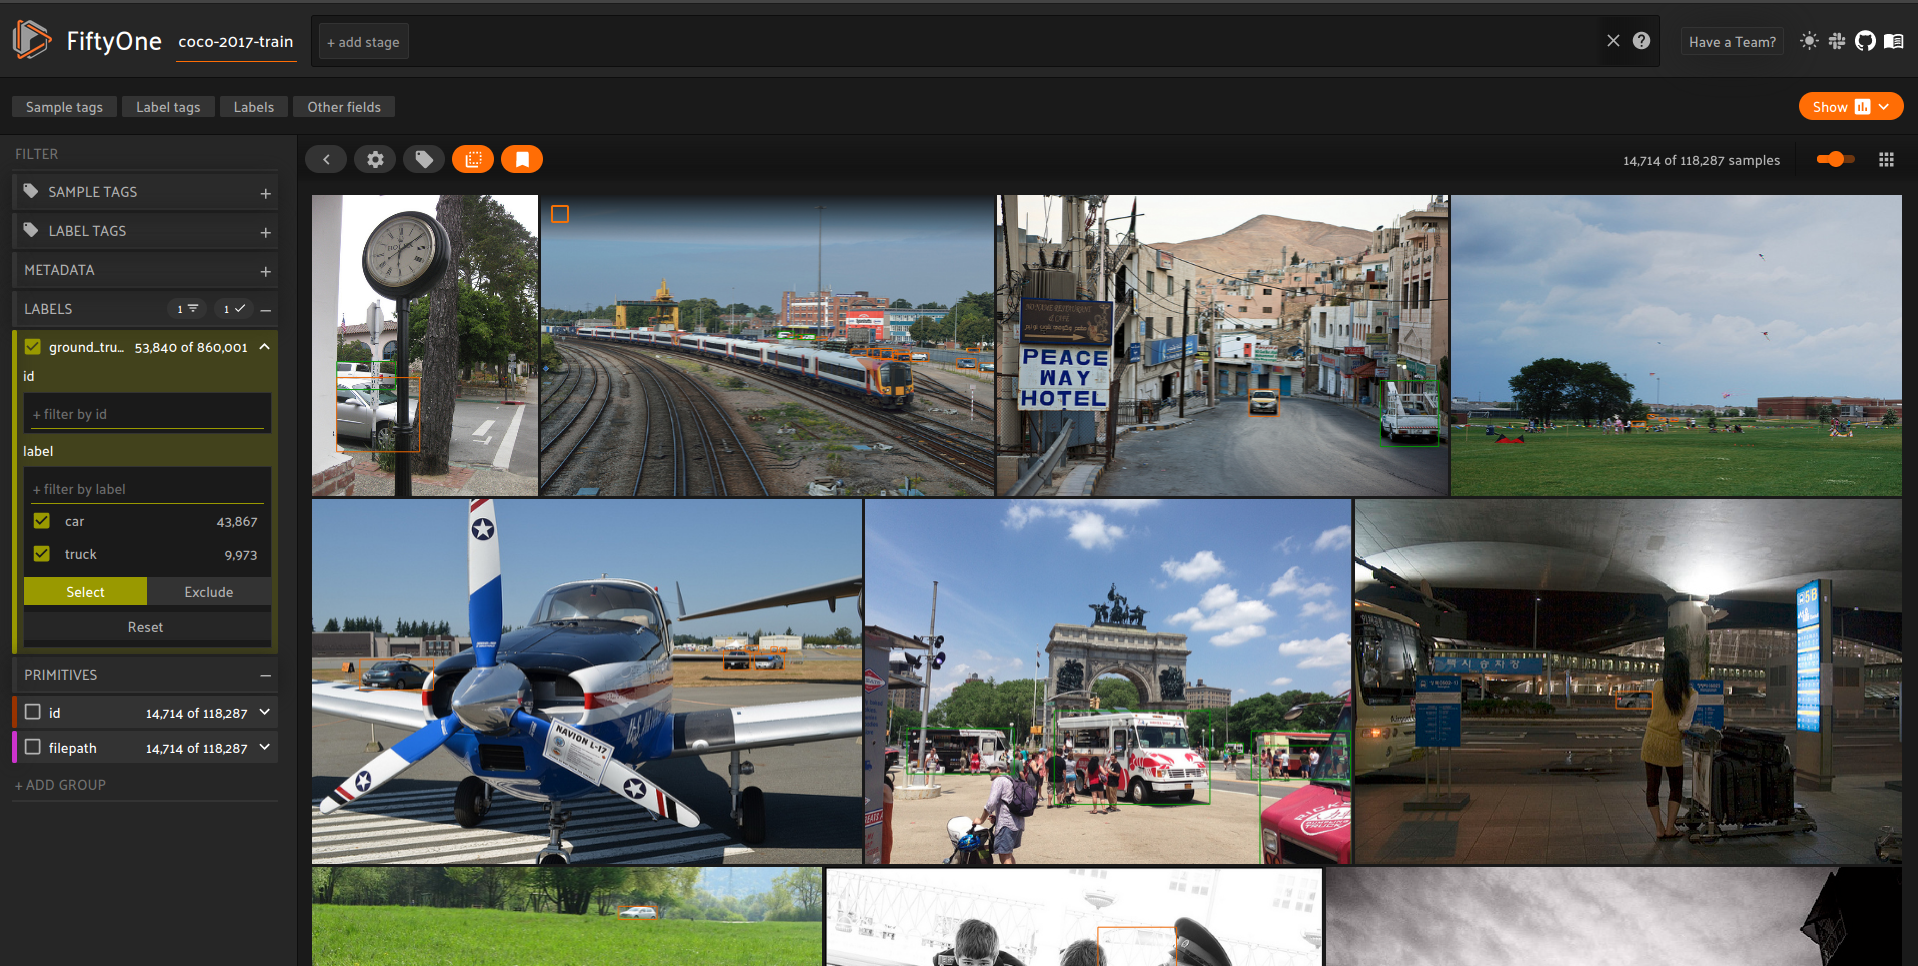
\includegraphics[width=\textwidth]{figures/fiftyone-coco-car-truck.png}
%     \label{fig:fiftyone-car-truck}
% \end{center}

\begin{figure}[h]
    \captionsetup{width=\textwidth}
    \caption{Exploring the train split of the MS COCO 2017 dataset in the FiftyOne tool. There are 43867 instances of labeled cars and 9973 instances of labeled trucks, with 14714 images containing either of them.}
    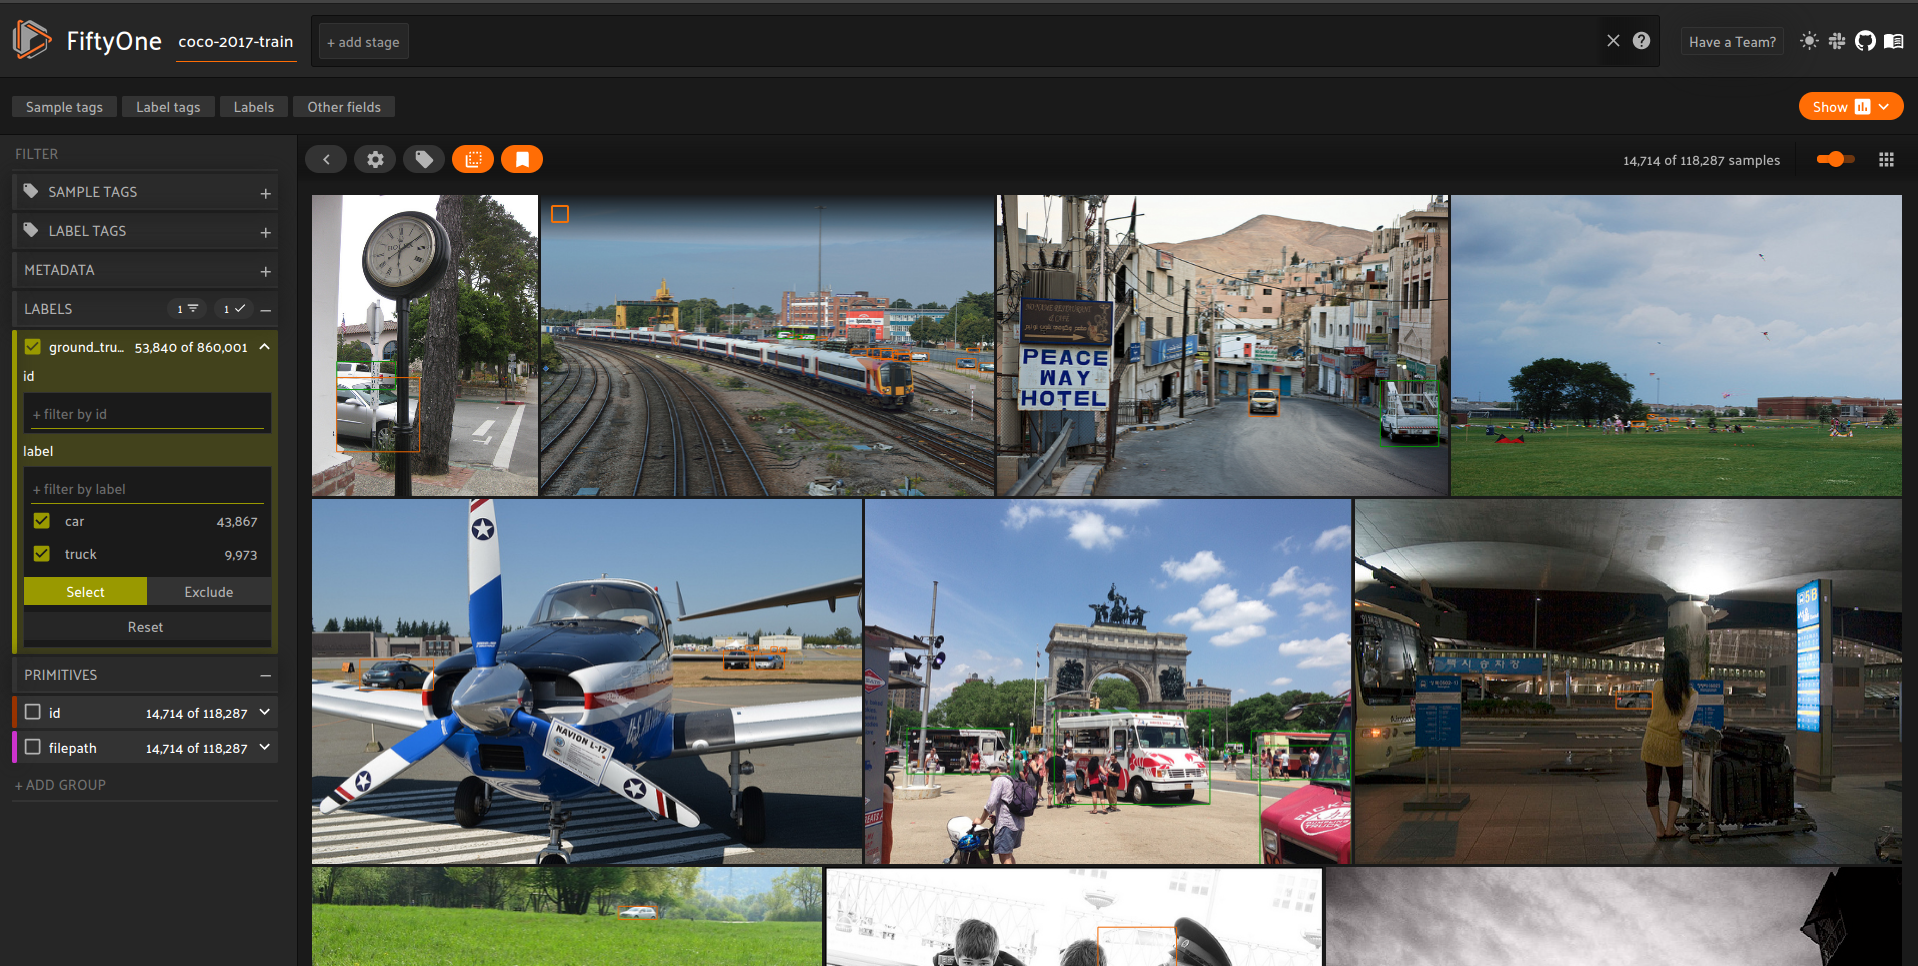
\includegraphics[width=\textwidth]{figures/fiftyone-coco-car-truck.png}\label{fig:fiftyone-car-truck}
\end{figure}

\begin{figure}[h]
    \captionsetup{width=\textwidth}
    \caption{Some difficult examples: objects in overexposed regions of the image, crowd labels consising of very small (e.g aerial) images of cars (orange) and trucks(green)}
    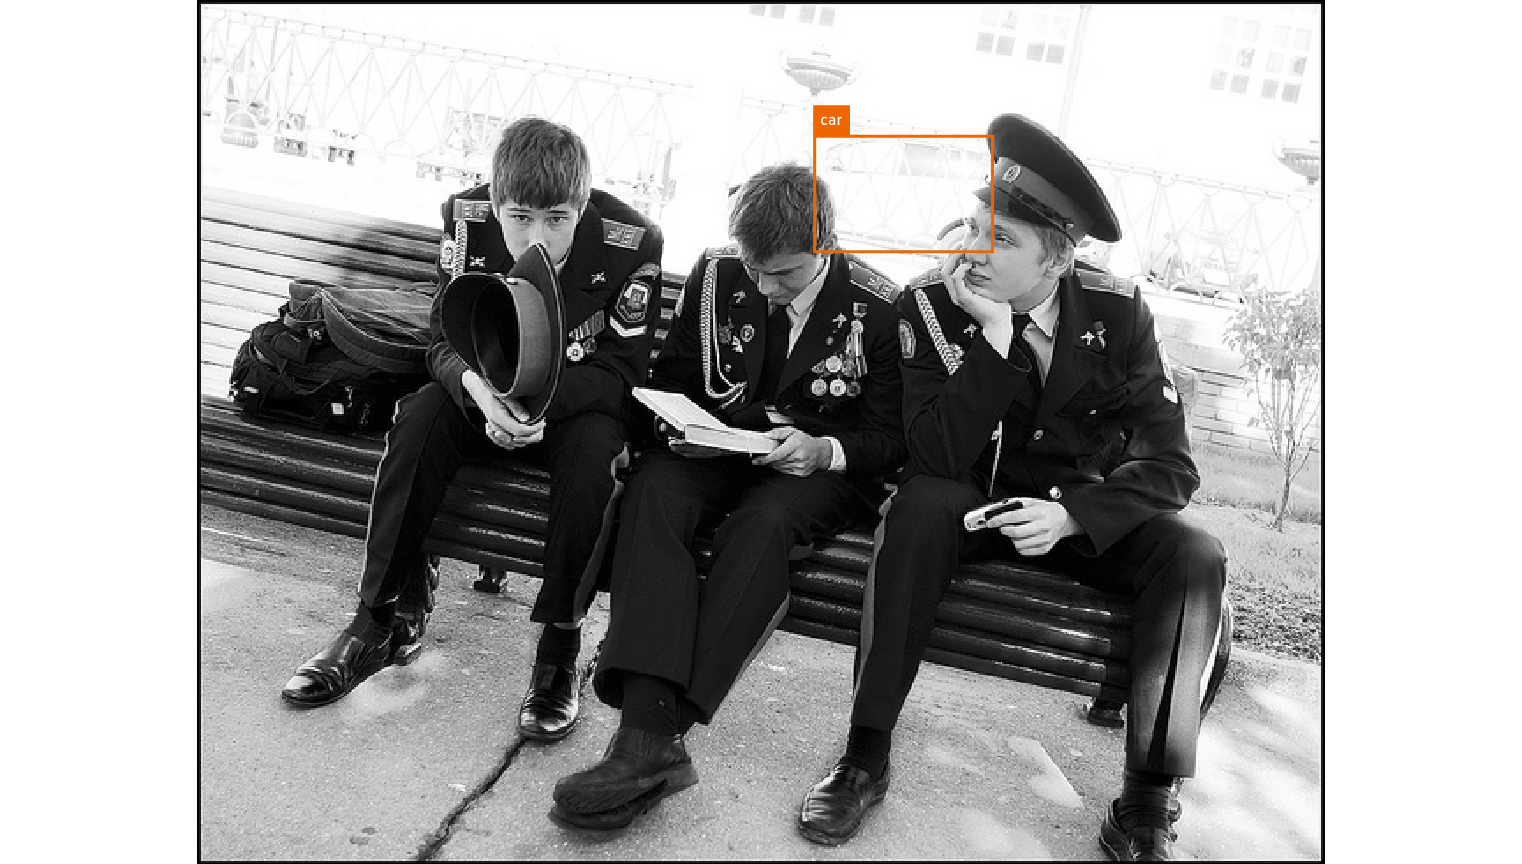
\includegraphics[width=.49\textwidth]{figures/car-overexposed.png}
    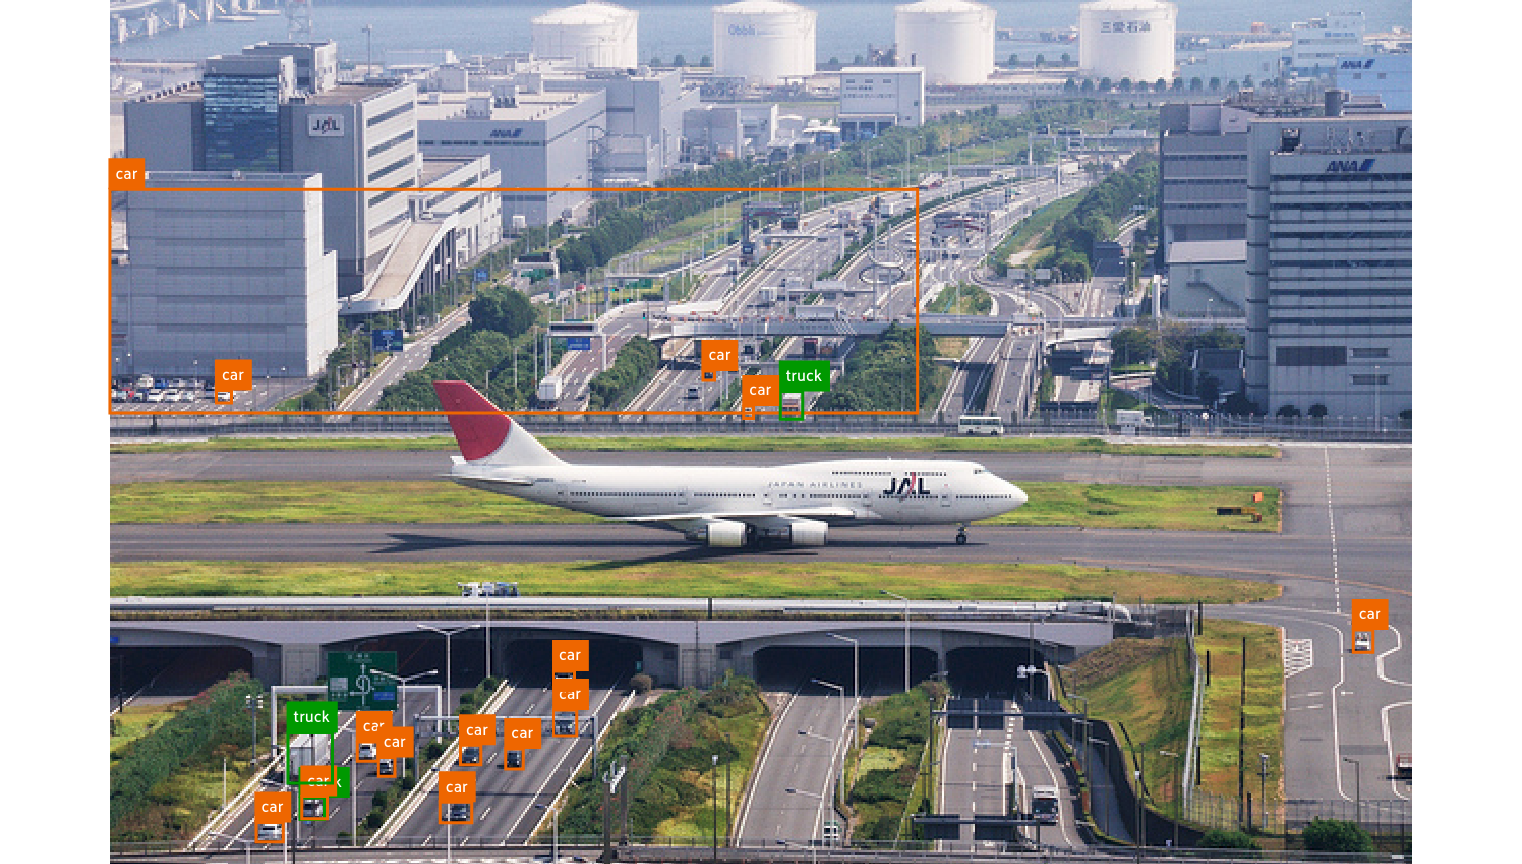
\includegraphics[width=.49\textwidth]{figures/car-truck-small-crowd.png}\\
    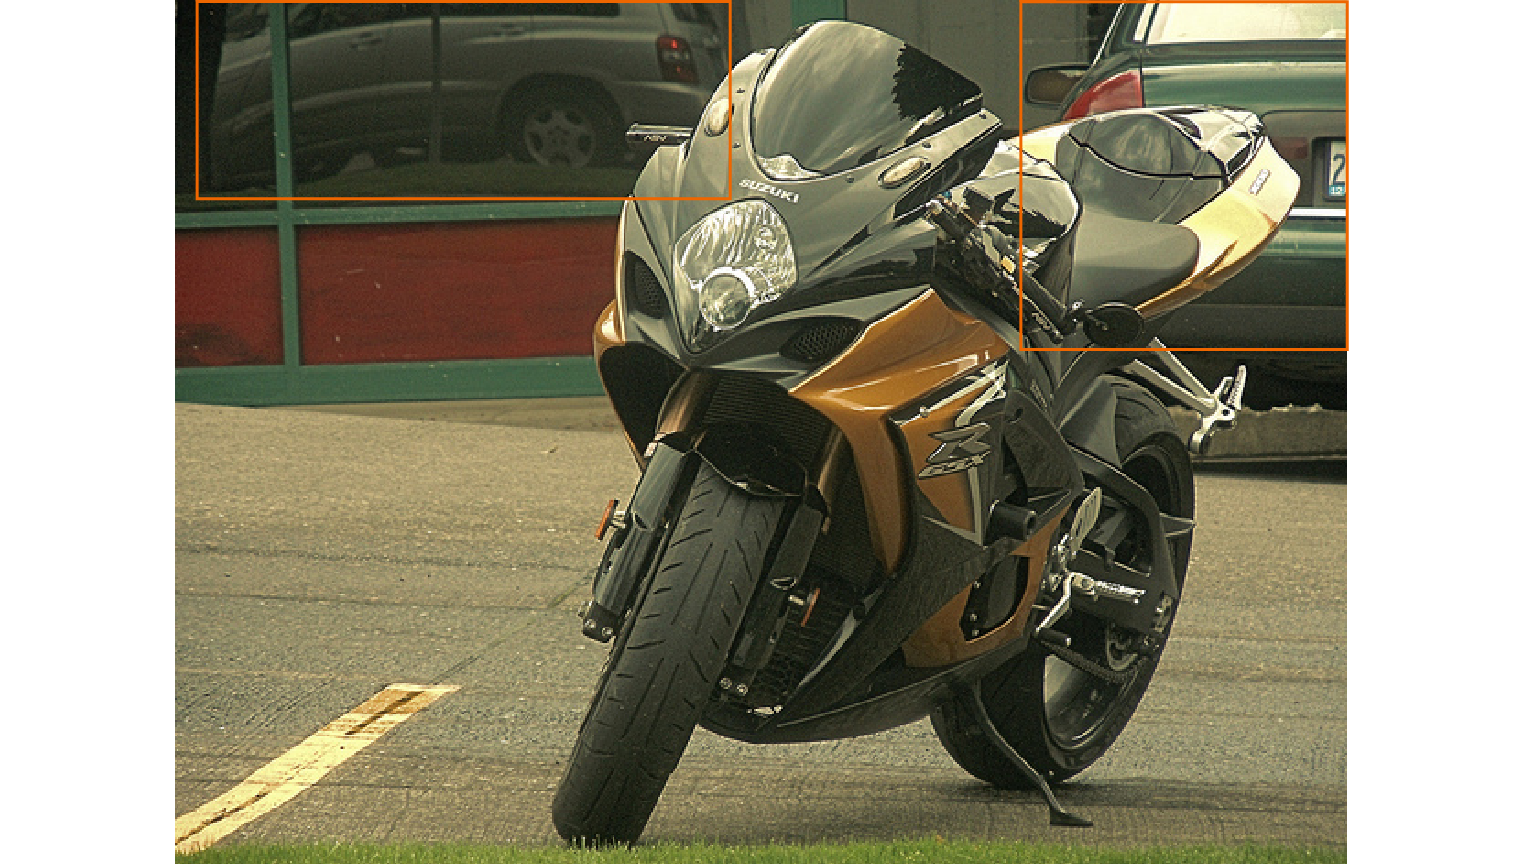
\includegraphics[width=.49\textwidth]{figures/car-reflection-partial.png}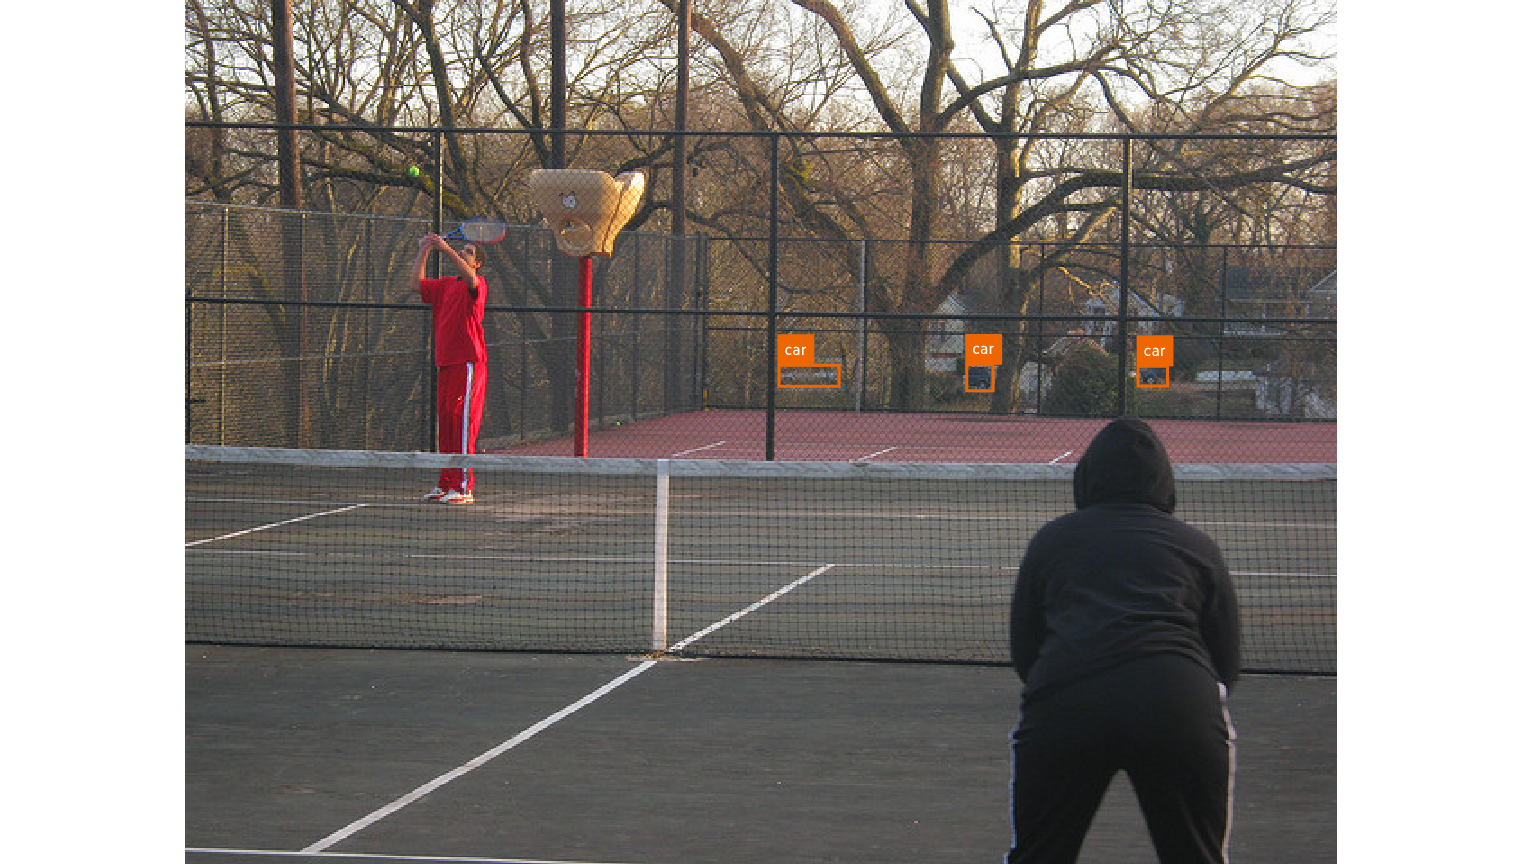
\includegraphics[width=.49\textwidth]{figures/car-obscure.png}\\
\end{figure}

% \subsection{kitti}




% \section{Training via Transfer Learning}

% \subsection{DETR}

\chapter{Evaluation on Multiple Object Tracking}

As the final aim of my thesis, I am going to inspect the performance of the chosen object detectors on a higher-order problem (meaning that detection is only the first conceptual layer of the solution), namely multiple object tracking (MOT). First I am going to review the problem itself, and the common metrics used to measure its performance. 

After this, I will elaborate on the object tracker implementation I chose as the basis, showing how it incorporates the aforementioned detectors, and the way the performance of the latter is expected to influence tracking performance.

Finally, I will describe my experimental setup aiming to measure tracker performance based on the detector type supplied to it. Several parts of the evaluation environment were implemented by me, so I will detail my design chices whenever such a part comes into focus.

\section{The problem and possible approaches}

Multiple object tracking (MOT) consists of determining the \textit{trajectory} of given kinds of objects in a video stream. In the current context, the trajectory of a single, unique object is a series of bounding boxes with an identifier, one box for every frame in which the object is visible. The rectangular bounding boxes are expected to fit the object shilouette as tightly as possible.

Along the years, several approaches have been developed for the problem, but with the advent of highly accurate object detectors (most notably the breakthrough of convolutional neural networks from the mid-2010s and onward), the detection-based paradigm has become one of the most popular.

The approach consists of detecting objects on each new frame, then assigning them to previously found trajectories, if the object has been seen before, or registering a new trajectory otherwise. This is generally called the \textit{association step}. In some scenarios, when the objects of interest are densely packed, this can pose a considerable difficulty.

Among some popular solutions to this association problem are the \textit{proximity-based} (the Simple Online and Realtime Tracking (SORT) architecture~\cite{Bewley_2016} is one example) and the \textit{feature-based} (the DeepSORT architecture \cite{DeepSORT} incorporates such methods using \textit{deep appearance descriptors}) assignments. The former considers each already existent trajectory, takes their previous location, or the predicted location for this time step, and does the assignment based on some spatial distance between these and current detections. The latter does overarching associations based on visual appearance features, not necessarily restricted to the appearance observed in the last few frames.

The weakness of the proximity-based approach is when the density of objects is high, their movement highly dynamic and their trajectories intertwined. In this case, feature-based methods might excel. The weakness of the feature-based methods might show when they confuse similar, but distinct objects, or when they cannot account for some drastic, fast changes in appearance (like changes in lighting, orientation, deforming, or partial occlusion). In these situations, assignment to last known locations can help. Thus, these two approaches are not, and should not be exclusive.

The introduction above focuses on paradigms and aspects mostly relevant for my thesis, and narrows down the field somewhat. For a comprehensive, recent overview of the problem, see the literature review at~\cite{Luo_2021}. It goes beyond just the detection-based approach, and also formalises the general problem.

Finally, it is worth mentioning that the most common multi-object tracking targets are pedestrians, faces and vehicles, and thus most popular MOT datasets consist of these. In this thesis, I am going to tackle tracking vehicles in road traffic footages.

\section{Metrics}

When thinking about assessing the performance of multiple object tracking applications, there is no one singular metric that comes to mind, but there are several ways in which a tracker can be wrong (at least in as many ways as an object detector). Starting from these errors, categorizing and counting them, and then inspecting their relation to the total of ground truth detections can give the right picture.

After inspecting some research literature in MOT, I saw that the most popular metrics coming up again and again were the CLEAR MOT metrics, or at least some of them. They were introduced in~\cite{Bernardin2008}, back in 2008, when generally-agreed upon metrics were not estabilished in the field. It proposes the MOTA and MOTP metrics as a way to quantify identity tracking and localization performance.

The CLEAR MOT paper provides not only the metrics themselves, but also explains the specifics of the evaluation process. After a literature and research review, it starts by defining the characteristics of a desirable tracker: `It should at all points in time find the correct number of objects present; and estimate the position of each object as precisely as possible (note that properties such as the contour, orientation, or speed of objects are not explicitly considered here). It should also keep consistent track of each object over time: each object should be assigned a unique track ID which stays constant throughout the sequence (even after temporary occlusion, etc.)'.

The proposed evaluation procedure should, in short, find best one-to-one assignment between object hypotheses (system predictions) and ground truth objects (usually in the form of bounding boxes with object identifier, using some distance metric for their dissimilarity) at every time step, and assess how well it went. First, I mention that I will use terms `object', `track', `prediction', `hypothesis' etc. interchangeably, but will usually use the term `track' when I consider its predicted identity, not only its location.

One kind of problem that can arise during assignment is that the hypothesis has no reasonably close match (denoted as some distance threshold T). Here, we talk about a \textit{false negative} (FN). Another problem can be that after assigment, predictions were left with no ground truth match. This can be because they are further away from any ground truth objects than the treshold, or simply there are more predictions than ground truth. Here we talk about a \textit{false positive} (FP). Until now, the metrics are the same as in the case of object detection.

One difference in evaluating though is the case of ambiguity: what happens if more predicted objects are within distance threshold? In the case of detection, usually the closest one is assigned, and if two ground truths share a single `closest' hypothesis, the Hungarian algorithm for bipartite graph matching solves this problem in a globally optimal way. In the case of tracking however, one must account for the identities of the objects.

When ground truth object A was previously assigned to predicted object X, then in the next step, two or more predicted objects are within ditance threshold to A. In the simplest case, if neither are X, the track is considered lost (or maybe prediction for X has wandered too far), another assigned track with a different identity will take its place through an identity swap, and it is a \textit{mismatch}. Otherwise if X is among them, and it is the closest one, then again, the assignment is simple. But when X is not the closest, we still assign it to A over the closest prediction, because we want to keep track identity for as long as possible, and it is the best approach to cases when the trajectories of the two objects overlap: if the prediction of one gets slightly closer to the other's ground truth, assigning by closest match would make us record an identity swap between the two, even though in reality both predictions were fairly good, staying within threshold.

Let $GT_t$ denote the number of ground truth boxes in a time step $t$, $FP_t$ the number of false positives, $FN_t$ the number of false negatives, while let $IDS_t$  denote the number of mismatches ($IDS$ is for identity switch, a notation used for the same concept in other publications, like~\cite{MOT15}). Then the first metric proposed by the paper is:

\[ MOTA = 1 - \frac{\sum_{t}{FP_t} + \sum_{t}{FN_t} + \sum_{t}{IDS_t}}{\sum_{t}{GT_t}} \]

The other one is $MOTP$, defined as \textit{the average dissimilarity between all hypothesis to ground truth assignments, across all time steps}. In this thesis, I will use the Intersection over Union (IoU) metric for box dissimilarity, or `box distance'.

\section{SORT}

Simple Online Realtime Tracker (SORT) was introduced in~\cite{Bewley_2016}, it is a simple yet very popular tracker implementation, presented as performing on par with state-of-the art solutions at the time. It is a detection-based tracker, and uses only positional information for the detection-to-track assignment, appearance features are ignored.

The tracking method is the following: at each step, the system keeps track of the objects already being tracked, as well as their last known position and velocity. The velocity is a computed value that comes from the difference in time of previous positions, but it is also smoothed by a Kalman filter. It predicts the expected next position and velocity based on the Kalman tracker's state, and when detections arrive, it makes a minimum-distance assignment between expected positions of the tracks and detections, using the Hungarian algorithm, and update the state of the tracks with the assigned detections.

If a previous track has no detection assigned, we keep predicting its possible next states to the extent of a parameter called \textit{maximum age}, then if a viable assigment arises, we keep tracking and reset \textit{maximum age}. If it is not reassigned by the time \textit{maximum age} reaches 0, the track is discarded.

If a prediction has no previous track assigned, we initialize it as a potential track. A given number (\textit{minimum hits}) of successive detection assigments to this potential track are needed to establish it as an actual track.

At the end, the Kalman filter self-corrects with the actual positions based on the assigment. In summary, the role of the Kalman filter is to provide possibility to infer hidden state (velocity, needed for prediction) from observable state (positions), provided a linear relationship between the two (\begin{math}\textbf{v}(t) = \textbf{s}(t)dt\end{math}), acting as a linear estimator for the trajectory.

The introduction to the paper states that the problem of occlusion (or brief loss of detection) is ignored for simplicity, but in the short term, it can be remedied by setting \textit{maximum age} properly.

For this project, I am using the official implementation\footnote{\url{https://github.com/abewley/sort}}.

\section{A popular benchmark}

In this section I will refer to one of the most popular multiple object tracking benchmarks, the MOT15, as well as its later versions, the MOT16, MOT17 and MOT20. It was introduced in~\cite{MOT15}, allong with the MOTChallenge\footnote{\url{https://motchallenge.net/}}. The metrics used in evaluation are the CLEAR MOT metrics. \cite{MOT15} defines a data format for saving detection and tracking results. The data should be stored in text files, with each line looking like:

\begin{table}[h]
    \centering
    \begin{tabular}{c c c c c c c c c c}
        \textit{frame} & \textit{ID} & \textit{x} & \textit{y} & \textit{w} & \textit{h} & \textit{conf.} & \textit{NA} & \textit{NA} & \textit{NA} \\
        1, & -1, & 794.2, & 47.5, & 71.2, & 174.8, & 67.5, & -1, & -1, & -1 \\
    \end{tabular}
\end{table}

\begin{table}[h]
    \centering
    \begin{tabular}{c c c c c c c c c c}
        \textit{frame} & \textit{ID} & \textit{x} & \textit{y} & \textit{w} & \textit{h} & \textit{conf.} & \textit{NA} & \textit{NA} & \textit{NA} \\
        1, & 3, & 875.4, & 39.9, & 25.3, & 35.0, & 0, & -1, & -1, & -1 \\
    \end{tabular}
\end{table}

The first one is from a detection file, the second one from a tracking annotation file. Here, frame is the number of the frame, ID is the identifier of th object, -1 in detection files. The next four entries are the box coordinates specifying the top left corner of the box, its width and height, the next is detection confidence (irrelevant for tracker annotation files).

The last 3 entries are not used in the output of either the detector or the tracker, but in the tracking ground truth files that the MOTChallenge uses to evaluate submitted results. They indicate certain objects that should not be tracked, or if tracked, should be ignored at evaluation. These objects include occluders, the reflections of the objects (which can be, but are not required to be found by the tracker, and the result should not be penalized either way).

I refered to this format because the official SORT implementation uses this as both input and output format, so it will be relevant information at the data processing steps.

\section{Choosing the data}

I will evaluate the model's performance for multi-object tracking on the UA-DETRAC dataset\footnote{\url{https://detrac-db.rit.albany.edu/}}. The dataset contains 100 videos (60 for training, 40 for testing) of road traffic captured at different locations in China. The total length of the video footage is around 10 hours, stored frame by frame (as separate 960 pixel by 540 pixel JPEG images), at the rate of 25 frames per second.

The annotations contain information about vehicle type, illumination, scale (proportional to the square root of the bounding box area), occlusion ratio (the measure by which other objects occlude the vehicle) and truncation ratio (the degree of the bounding box lying outside the frame). Information about weather conditions e.g.~rainy, cloudy, sunny etc.~is also included.


\section{Data Exploration}

At the time of writing this thesis, the test and train images, grouped into sequences that form videos, can be accessed through the Download page of the official site\footnote{\url{https://detrac-db.rit.albany.edu/download}} as \verb|DETRAC-train-data.zip|. However, the tracking annotations for the train and test sets cannot be downloaded, as clicking on the links triggers a popup prompting to log in first. As the login functionality currently does not work, I had to look for alternative ways to access the data.  

Fortunately, after a short search I have found a GitHub repository owned by the Georgia Tech Database Group. Their Exploratory Video Analytics System (EVA) repository contains, among others, a guide on how to download the UA-DETRAC dataset\footnote{\url{https://github.com/georgia-tech-db/eva/tree/master/data/ua_detrac}}, along with a bash script serving the same purpose.

Through those links, I could download the training annotations. Sadly, the test annotations, claimed on the official UA-DETRAC website to be released, were still nowhere to be found, but I figured the 60 sequences (or even a subset of them) should be enough to evaluate tracking performance. The integrity of the measurement wouldn't have been compromised either, as I wasn't planning on doing detector training or hyperparameter tuning on the train set. There were two kinds of training annotation formats provided: XML and MAT.

The XML annotations are meant for detection training, and contain additional information like vehicle category, weather conditions during filming and bounding box scale. I did not use this data directly, as I used the models pre-trained on the COCO dataset, but inspecting this data confirms the vehicle categories supported by the DETRAC dataset: \textit{car}, \textit{van}, \textit{bus}, \textit{other}. The corresponding COCO object categories are \textit{car}, \textit{truck}, \textit{bus}, so that is what I will be looking for when runnning detection on the images, and ignoring all other classes.

The MAT annotations are files in MATLAB serialization format, containing trajectory and position information for all tracked entities. For every image sequence, there is a \verb|MVI_NNNNN.MAT| file.
The image sequences themselves are consecutive frames under \verb|Insight-MVT_Annotation_Train/MVI_NNNNN|, after unzipping \verb|DETRAC-train-data.zip|.

Initially I inspected the MAT files' inner structure (see figure~\ref{fig:octave-exploration}) in GNU Octave, MATLAB's open-source and somewhat compatible counterpart. I found that each file contained 5 matrices:
\begin{enumerate}
    \item{$X$: An $N \times T$ matrix, where $T$ is the number of trajectories, and $N$ is the number of frames. Given the frame $i$ and trajectory $j$, $x_{i,j}$ denotes the $x$ coordinate of the bottom center of the bounding box\footnote{I found this out initially through trial and error, when trying to visualize bounding boxes in Python, because I did not know this to be a common format for specifying bounding boxes. Later, I found it mentioned in \url{https://detrac-db.rit.albany.edu/FAQ} as \textit{foot position}.}, or $0$ if trajectory $j$ is not present in that frame.}
    \item{$Y$: An $N \times T$ matrix, similar to $X$, but it contains the $y$ coordinates of the bounding boxes' foot position.}
    \item{$W$: contains the width of the boxes.}
    \item{$H$: contains the height of the boxes.}
    \item{$frameNums$: A row vector of length $N$, containing the 1-based indices of the frames.}
\end{enumerate}

\begin{figure}[h]
    \begin{center}
        \captionsetup{width=0.8\textwidth}
        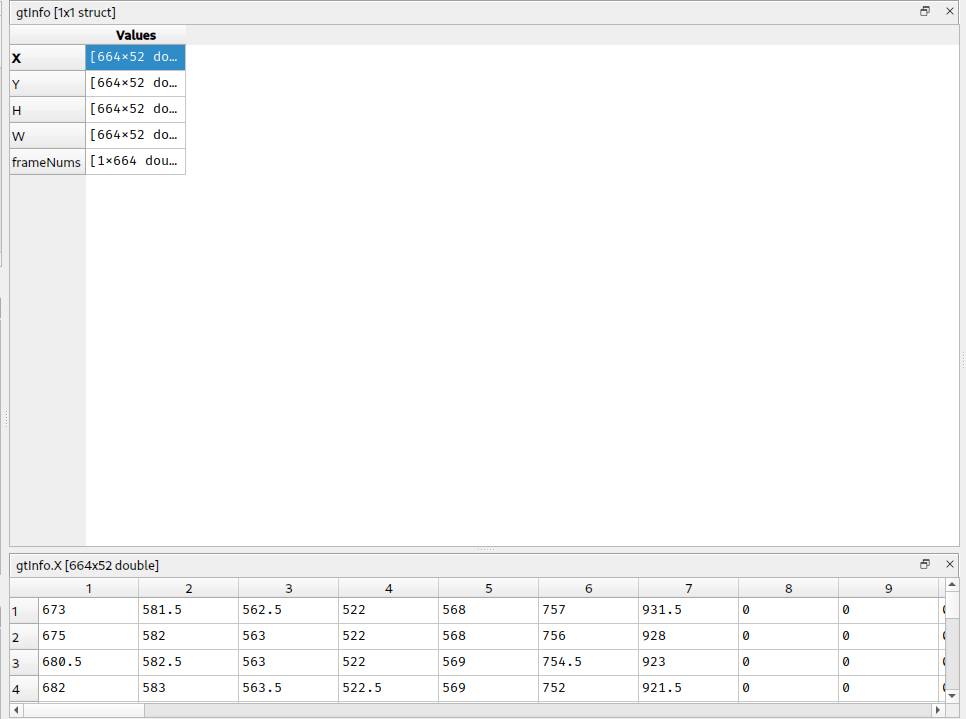
\includegraphics[width=0.8\textwidth]{figures/octave.png}
        \caption{Label data exploration in octave}
        \label{fig:octave-exploration}
    \end{center}
\end{figure}


\section{Used benchmark}

The dataset and the benchmark is described in~\cite{CVIU_UA-DETRAC}. The article also proposes an evaluation protocol for multi-object tracking. A key point is the joint analysis of detection and tracking performance, analysing the effects of the chosen model's precision/recall values (and the underlying confidence threshold setting that influences both) in relation with the tracking performance, as reflected by the MOTA and MOTP score. These relationships are visualized on the PR-MOTA and PR-MOTP curves (See figure~\ref{fig:pr-mota}).

\begin{figure}[h]
    \captionsetup{width=\textwidth}
    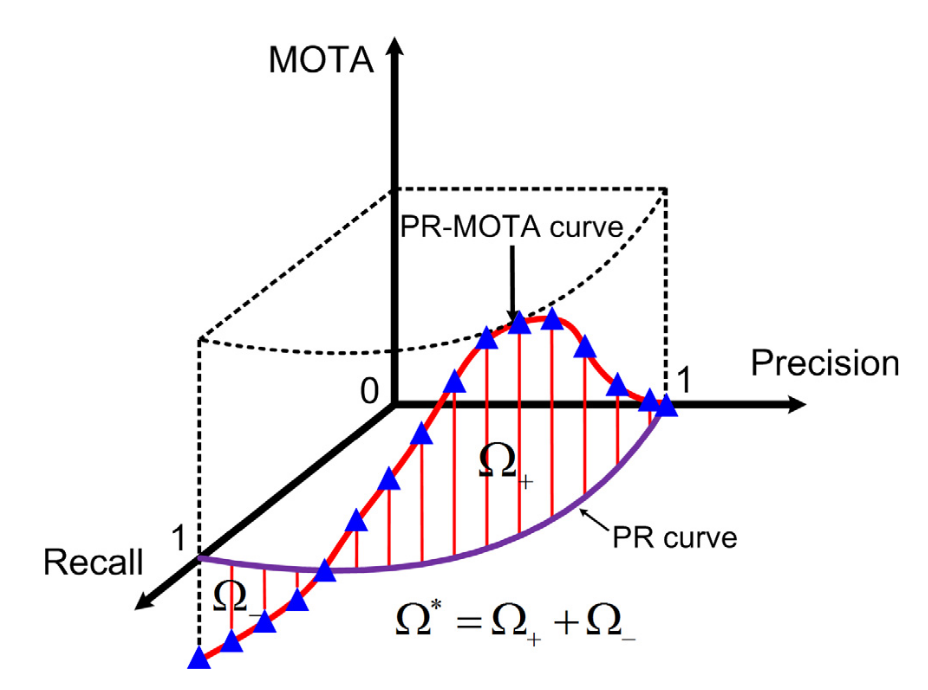
\includegraphics[width=\textwidth]{figures/pr-mota-curve.png}
    \caption{Visualization of the PR-MOTA curve. Image taken from \cite{CVIU_UA-DETRAC}}
    \label{fig:pr-mota}
\end{figure}

The authors argue that, as it is not fair, nor enough to compare the performance of two object detectors based on different points on the PR curve, it is also not enough to determine the maximum point on the PR-MOTA curve, as a good tracker must produce good scores in a wider range of settings. The whole range of the curve must be taken into account in some form, thus the need for a new metric, $\Omega^{*}$, or the \textit{PR-MOTA score}:

\[ \Omega^{*} = \frac{1}{2}\int_{\mathcal{C}} \Psi(p, r) \,d\textbf{s} \]

where $\Psi$ is the MOTA score across the whole dataset at precision $p$ and recall $r$, and we calculate the (approximate value of the) signed area under the PR-MOTA curve as an integral along the PR curve $\mathcal{C}$ (for every $(p, r) \in \mathcal{C}$). Dividing by 2 ensures that the score stays in the interval $(-\infty, 100\%]$. Similar metrics can be defined for the MOTP, FP, FN, IDS, MT and ML scores.

\section{Designing the measurement}

For the measurment, I chose 7 detectors in total: two DETR variants, one with the ResNet50 and one with the ResNet101 backbone, pre-trained on the COCO 2017 dataset. The other 5 were the YOLOv5n (nano), YOLOv5s (small), YOLOv5m (medium), YOLOv5l (large), YOLOv5x (extra large). These differ in the size, as in number of parameters, and this influences the inference times as well.

Each detector was evaluated at 10 confidence thresholds: from 0.0 to 0.9, incremented by 0.1.

To calculate the value defined by the UA-DETRAC benchmark, I had to break the process into multiple steps and assess the best tool for each subtask.

As input data, I had the UA-DETRAC training videos, as frame sequences, and the annotations in MATLAB format.

For my tracker of choice, I could clone the public GitHub repository\footnote{\url{https://github.com/abewley/sort}}, and run the tracker, provided I put the detections in MOT2015 format for each sequence under the \verb|data| folder.

The rest of the steps had to be implemented by me. First, I had to create a model executor that returned the detections from each frame of the video sequences, and served as a adapter-wrapper around both the DETR and the YOLOv5 models, to hide the differences in preprocessing. I invoked this this on all combinations of models, confidence thresholds and sequences. For each unique trio of these, one file has been saved in the MOT15 detection format.

The detections themselves, along with the annotations were enough to calculate the precision-recall curve for each model, aggregating the values for all sequences. For evaluation I used the standard IoU metric for ground truth-prediction distance, with IoU threshold 0.7 (In the code, \verb|max_iou| is set to 0.3, because the library I used considers $1-IoU$ when matching ground truth with prediction. More on that in the relevant subsection). This is not to be confused with the confidence threshold, which is a property of the detector that can be set, and varies. This is a global setting which means that a good prediction can be considered a match to the ground truth box only if their IoU distance is at least 0.7, a reasonable expectation according to my visual intuition.

Next, I ran the SORT script provided in the official repository for each model separately, on every sequence and confidence threshold combination. These were automatically saved in the MOT15 tracking annotation format.

Having the tracking output and the ground truth annotations, I ran the tracking evaluation on every model and confidence threshold combination, aggregating MOTA values for all sequences. The evaluation IoU threshold was set to 0.7, like at the detection evaluation.

Given both the precision-recall curves for every model (where both precision and recall are a function of the confidence threshold), and the MOTA values for every model and confidence threshold combination, I could finally calculate the PR-MOTA scores for each model.

A visual overview of the process above can be seen in figure~\ref{fig:workflow}. Detailing of the individual design choices made at each step can be found in the following subsections. At some of the steps, I implemented visualizations as a way to spot possible errors in implementation that could compromise the whole measurement. 

The language I used was Python 3.10, the inference times were recorded under Linux, on a desktop PC with an AMD Ryzen 3800X processor, 32 Gigabytes of RAM and an RTX3060Ti graphics card with 8 Gigabytes of VRAM. 

\begin{figure}[h]
    \captionsetup{width=\textwidth}
    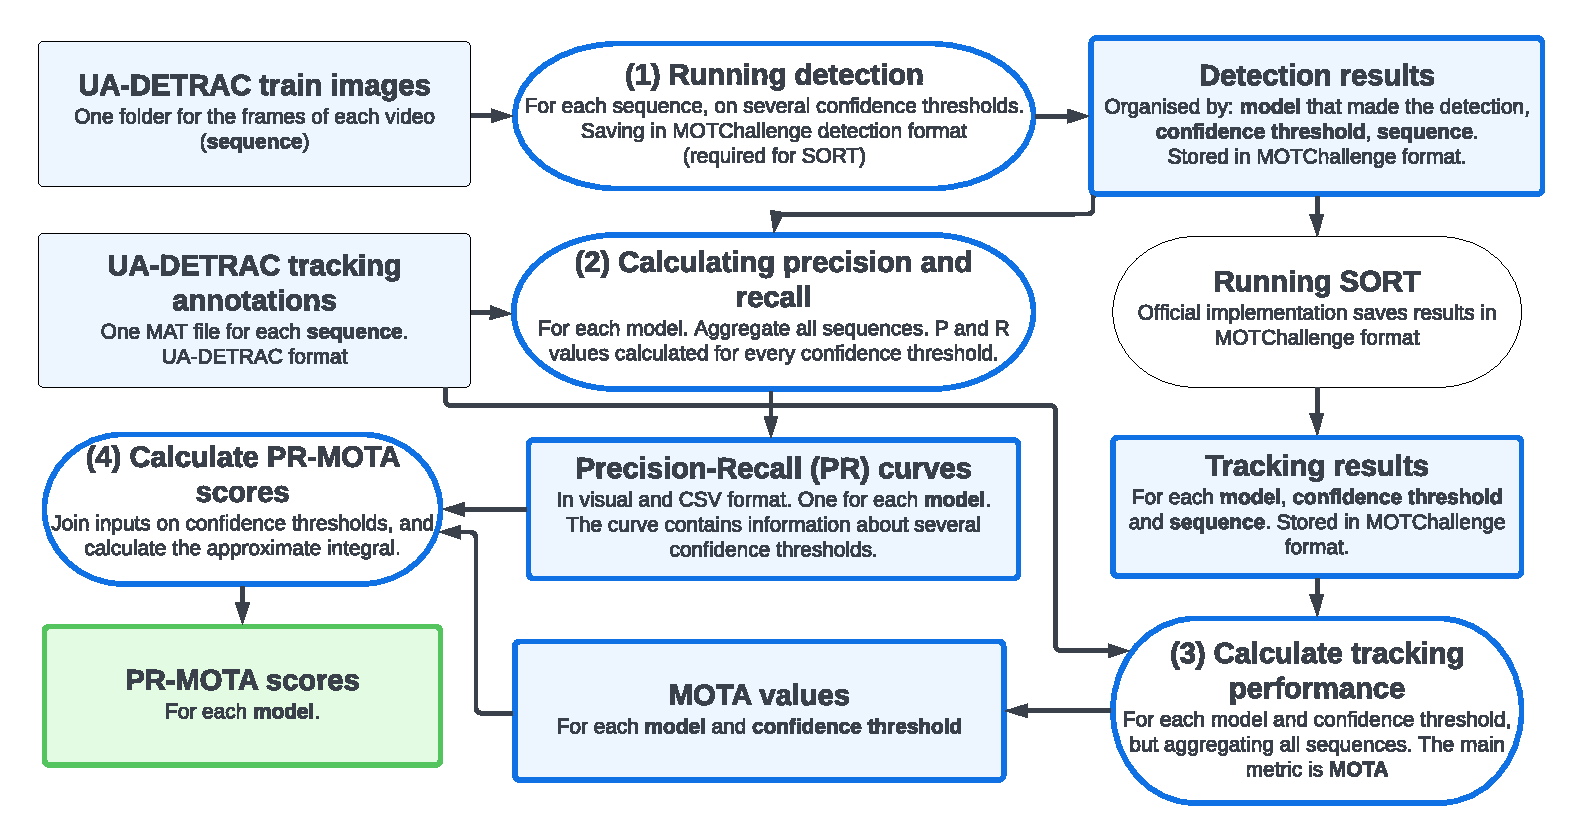
\includegraphics[width=\textwidth]{figures/workflow.pdf}
    \caption{Flowchart visualization of my workflow. The blue rectangles denote data, rounded rectangles denote processing steps. Blue outline means that part of the workflow was implemented by me, or the data was generated in the process. No blue outline means either the data is from an external source, or the processing step involved using entirely external code.}
    \label{fig:workflow}
\end{figure}

\subsection{Running the detections}

In order to evaluate the aforementioned models on images, I had to find the easiest way to load the pretrained weights for each model.

For the DETR, the \verb|transformers| Python package by Huggingface\footnote{\url{https://huggingface.co/docs/transformers/index}} provides the easiest API, with simple pre- and postprocessing (including confidence thresholding and converting from logits to probability distributions), and also provides a way to download pretrained weights. Under the hood, \verb|transformers| uses a PyTorch \verb|torch.nn.Module|, so sending it to the GPU is similar to all Torch modules. Also theoretically loading from Torch Hub was also a possibility, but the pre- and postprocessing tasks would have been messier.

As for the YOLOv5 model, it can be loaded directly from Torch Hub, and its input format is way more flexible, so lists of images (for the inference, I used batches of size 1), but even image links can  be fed to it directly.

To hide the differences between these two approaches, I implemented an adapter class for them, and also added visualization capabilities to spot possible errors in the interpretation of data (for example, assuming wrong bounding box format).

I also wanted to meausre average inference times to show a picture about the real time capabilities of each detector. All inference happened on the GPU, so due to the asynchronous nature of the Torch CUDA operations, measuring elapsed time on CPU was out of the question. The appropriate time measuring method, as suggested on the official Torch forums\footnote{\url{https://discuss.pytorch.org/t/how-to-measure-time-in-pytorch/26964}} was through the \verb|torch.cuda.Event| object. I took the elapsed GPU time between the moment of feeding the inputs until recieving the logits, but this didn't include copy times between the RAM and VRAM, neither the postprocessing steps (calculating probability distributions with softmax, confidence thresholding).

Timing results can be seen in table~\ref{tab:inference-times}. All code to reproduce the results can be found on the GitHub repository of my thesis\footnote{
    See \url{https://github.com/peter-i-istvan/bsc-thesis}, under \texttt{tracking/run\_detection.py}.
}.

\begin{table}[h]
    \begin{tabular}{|c|c|c|c|c|c|c|c|}
        \hline
         & yolov5n & yolov5s & yolov5m & yolov5l & yolov5x & detr-resnet-50 & detr-resnet-101 \\
        \hline
        \hline
        avg (ms) & 7.38 & 7.38 & 8.99 & 12.00 & 20.88 & 43.98 & 64.53 \\
        \hline
        std (ms) & 1.16 & 0.24 & 0.24 & 0.18 & 0.27 & 0.80 & 0.66 \\
        \hline
        \hline
            FPS & 135.5 & 135.5 & 111.2 & 83.3 & 47.89 & 22.73 & 15.49 \\
        \hline
    \end{tabular}
    \caption{Average inference times on GPU and their standard deviation (expressed in miliseconds) for each model, after running on every sequence.}
    \label{tab:inference-times}
\end{table}

\subsection{Calculating precision and recall}

Next, I had to calculate precision and recall curves for the detections. To do this, for every model and confidence threshold pair, I had to sum all true positives, false positives and false negatives in every sequence. For the theoretical definition of these, not only in the general meaning, but in the case of object detection, where assignment between ground truth and predicted boxes is not always trivial (the Hungarian bipartite graph matching algorithm solves this ambiguity), see chapter one.

For the concrete implementation, I took a `sideways' approach, but one that could be mostly reused later in calculating the MOTA score as well. The \verb|motmetrics| Python package\footnote{\url{https://pypi.org/project/motmetrics/}} provides handy tools for calculating MOT metrics, like those in CLEAR MOT. Specificaly, it gives us an \textit{accumulator} object that must be initialized before evaluating on a seqence, then for each frame, its \verb|update()| function must be called to update its state. In the arguments, one must provide ground truth IDs and predicted IDs, as well as a distance matrix that expresses the distance between ground truth box \textit{i} and prediction box \textit{j}. In theory, \verb|motmetrics| is distance-agnostic, which means that any kind of distance can be supplied, but I used the IoU box distance metric, which is one of the most popular evaluation metrics both for object detection and multiple object tracking. \verb|motmetrics| provides functions for calculating all popular metrics, so incorporating IoU calculation into my code was easy.

In its update step, the accumulator takes the input arguments, and in the first parts, it is not at all concerned with the IDs provided, but calculates the best ground truth box-to-prediction assignment with the Hungarian algorithm. This is the very exact action that is needed at detection evaluation as well, this is why we `piggy-backed' tracking evaluation. Based on this assignment, it generates \verb|MATCH|, \verb|MISS| and \verb|FP| events, which correspond to true positives, false negatives and false positives respectively.

In the next steps, if we provided valid prediction IDs (a.k.a our hypotheses for the identities of the tracked objects), the accumulator would also record possible mistakes with regard to identity confusion, like identity swaps. However, considering that the MOTChallenge format defines -1 as the ID field when saving only detections, not tracking results, technically we tell the accumulator that all found boxes correspond to our object -1, which makes the rest of this step absolute rubbish, but it does not influence the events already recorded in the first step, and in the first steps of all future update calls.

After finishing a sequence, the script extracts the number of relevant events, and adds them to all the previously calculated occurrences of true positives, false negatives and false positives for that model-confidence threshold pair. At the end of this, we will have a mapping counting all of these for every sequence. Then I iterate through all model-confidence threshold pairs, calculate the precision and recall values given by the formulas:
\[P = \frac{TP}{TP + FP}\]
\[R = \frac{TP}{TP + FN}\]

Finally, I save them as CSV files. The result can be seen in tables~\ref{tab:p_curve} and~\ref{tab:r_curve}.

\begin{table}
    \begin{centering}
    \begin{tabular}{|c||c|c|c|c|c|c|c|}
        \hline
        CT & D101 & D50 & YL & YM & YN & YS & YX \\
        \hline
        \hline
        0.9 & 0.52 & 0.47 & 0.93 & 1.0 & 1.0 & 0.90 & 0.64 \\
        \hline
        0.8 & 0.45 & 0.41 & 0.54 & 0.61 & 0.83 & 0.61 & 0.49 \\
        \hline
        0.7 & 0.40 & 0.37 & 0.54 & 0.51 & 0.68 & 0.52 & 0.46 \\
        \hline
        0.6 & 0.36 & 0.33 & 0.51 & 0.46 & 0.53 & 0.45 & 0.44 \\
        \hline
        0.5 & 0.33 & 0.30 & 0.46 & 0.42 & 0.42 & 0.39 & 0.41 \\
        \hline
        0.4 & 0.30 & 0.28 & 0.40 & 0.37 & 0.34 & 0.32 & 0.36 \\
        \hline
        0.3 & 0.28 & 0.26 & 0.33 & 0.31 & 0.28 & 0.27 & 0.30 \\
        \hline
        0.2 & 0.25 & 0.23 & 0.30 & 0.28 & 0.25 & 0.24 & 0.27 \\
        \hline
        0.1 & 0.21 & 0.21 & 0.30 & 0.28 & 0.25 & 0.24 & 0.27 \\
        \hline
        0.0 & 0.19 & 0.18 & 0.30 & 0.28 & 0.25 & 0.24 & 0.27 \\
        \hline
    \end{tabular}
    \caption{The precision curve of the models. CT is confidence threshold, D101 and D50 is DETR-Resnet 101 and 50, while YL, YM, YN etc. are the yolo versions.}
    \label{tab:p_curve}
    \end{centering}
\end{table}

\begin{table}
    \begin{centering}
    \begin{tabular}{|c||c|c|c|c|c|c|c|}
        \hline
        CT & D101 & D50 & YL & YM & YN & YS & YX \\
        \hline
        \hline
        0.9 & 0.63 & 0.57 & 0.03 & 0.01 & 0.00 & 0.02 & 0.12 \\
        \hline 
        0.8 & 0.69 & 0.65 & 0.41 & 0.34 & 0.13 & 0.36 & 0.46 \\
        \hline 
        0.7 & 0.71 & 0.68 & 0.59 & 0.52 & 0.41 & 0.56 & 0.60 \\
        \hline 
        0.6 & 0.73 & 0.69 & 0.69 & 0.63 & 0.52 & 0.66 & 0.69 \\
        \hline 
        0.5 & 0.73 & 0.71 & 0.76 & 0.72 & 0.60 & 0.72 & 0.76 \\
        \hline 
        0.4 & 0.74 & 0.71 & 0.81 & 0.79 & 0.66 & 0.77 & 0.81 \\
        \hline 
        0.3 & 0.75 & 0.72 & 0.84 & 0.84 & 0.70 & 0.80 & 0.84 \\
        \hline 
        0.2 & 0.75 & 0.72 & 0.86 & 0.86 & 0.72 & 0.81 & 0.86 \\
        \hline 
        0.1 & 0.76 & 0.73 & 0.86 & 0.86 & 0.72 & 0.81 & 0.86 \\
        \hline 
        0.0 & 0.76 & 0.73 & 0.86 & 0.86 & 0.72 & 0.81 & 0.86 \\
        \hline
    \end{tabular}
    \caption{The recall curve of the models. CT is confidence threshold, D101 and D50 is DETR-Resnet 101 and 50, while YL, YM, YN etc. are the yolo versions.}
    \label{tab:r_curve}
    \end{centering}
\end{table}

Running this took 1 hour and 8 minutes on my machine. For implementation, see my GitHub repository\footnote{See \url{https://github.com/peter-i-istvan/bsc-thesis}, under \texttt{tracking/detection\_evaluation.py} for the code, \texttt{p\_curve.csv}, and \texttt{r\_curve.csv} for the curves in }, where the curves are also available, saved in CSV format.

Finally, I wrote a small script that plots precision-recall curves\footnote{\url{https://github.com/peter-i-istvan/bsc-thesis} under \texttt{tracking/plot\_pr.py}. The PNG plots are also there under the root directory.} for each model. The results can be seen in figures~\ref{fig:pr_detr} and~\ref{fig:pr_yolo} in the appendix.

\subsection{Running SORT}

I ran SORT by cloning its repository, applying a small patch to account for divison by 0 at empty detection files (happened with YOLOv5n models for some sequences, at high confidence thresholds), installing the dependencies and issuing the following command:
\begin{verbatim}
    python sort.py --seq_path DETECTIONS_ROOT --phase MODEL --max_age 3
\end{verbatim}

The main hyperparameters of SORT are \verb|min_hits|, \verb|max_age| and \verb|iou_threshold|, all of them can be supplied to the script by command line parameters.

Minimum hits means the minimum number of consecutive times a new trajectory must be confirmed (by detection `hits' that get assigned to it) to consider it a real one. Its default value is 3, and I left it at that.

Maximum age is the longest consecutive time that a trajectory without detection (if the detector somehow lost the object) can be kept alive. The position predictions are still updated, so the tracker looks for the object a little bit further apart at each frame, in the direction and considering the magnitude of the last known velocity. The default value is 1, but I set it to 3 because it seemed reasonable (based on my experiences in the Project Laboratory course, where similar maximum ages lead to better results).

IoU threshold is the minimum IoU value between the hypothesized current bounding box location of the object (predicted by the Kalman filter) and any detection bounding box that can be matched with it. The default value is 0.3, and I left it at that.

During the consecutive runnings of the script, I recorded the elapsed time and FPS reported by the script for each model. The results are confirming the belief that SORT is a very fast tracker, with the main factor for the tracking framerate in a real time scenario (where detections are not precomputed) being the detection time (almost two orders of magnitude higher than the tracking time at each frame). For the results, see table~\ref{tab:sort-times}.

\begin{table}[h]
    \begin{tabular}{|c|c|c|c|c|c|c|c|}
        \hline
         & yolov5n & yolov5s & yolov5m & yolov5l & yolov5x & detr-resnet-50 & detr-resnet-101 \\
        \hline
        \hline
        Time (s) & 1313.99 & 1155.18 & 482.8 & 599.88 & 611.18 & 654.18 & 668.11\\
        \hline
        \hline
        FPS  & 637 & 725 & 1710.2 & 1391.7 & 1369.1 & 1279.1 & 1253.5 \\
        \hline
    \end{tabular}
    \caption{Statistics reported by the SORT script. The evaluation was done on 60 videos and on 10 confidence thresholds, making a total of 600 detection inputs. The time is the total evaluation time for all 600 inputs. The numbers are aggregated over confidence thresholds, but on lower values, tracking tends to take more time, as the consistent erroneus detections form a high number of false tracks.}
    \label{tab:sort-times}
\end{table}

\subsection{Calculating tracking performance}

After the tracking outputs were ready, I ran the tracking evaluation. The main goal was to calculate MOTA scores, average MOTA for every model-confidence threshold pair, across all sequences. Eventually I ended up calculating more metrics, to see a broader picture about the tracker performance.

For this, I used the \verb|motmetrics| library, similarly to the detection evaluation. I processed each sequence with an accumlator objects, computing several summary metrics at the end. For every model, confidence threshold, sequence trio, I had a summary in the form of a Pandas dataframe, holding all the same metrics. I gathered all these, then aggregated across the sequences, recieving aggregate scores for each model and confidence threshold.

The scores I queried in for each sequence were the \textit{MOTA}, \textit{MOTP}, number of \textit{identity switches}, the number of \textit{mostly tracked trajectories} (80\% or more of it was tracked), \textit{mostly lost trajectories} (20\% or less of it was tracked), and the number of \textit{unique objects}. I aggregated the MOTA and MOTP by averaging (also saving minimum and maximum MOTA score), the rest by calculating the sum of their values.

It is important to mention that I sticked to the original definition of MOTP, introduced in~\cite{Bernardin2008}, meausres average IoU dissimilarity between true positive predicted trajectories and ground truth, and a smaller value is preferable. In some publications, even in~\cite{Bewley_2016}, the value claimed to be MOTP is actually $1-MOTP$, scaled to percentages, so that higher value is better.

Running this took 1 hour and 10 minutes. For implementation, see the GitHub repository\footnote{\url{https://github.com/peter-i-istvan/bsc-thesis} under \texttt{tracking/tracking\_evaluation.py}. The results in CSV format are also available from the root directory of the repository, as \texttt{MODELNAME\_mota.csv}}. Results can be seen in tables~\ref{tab:mota_yn},~\ref{tab:mota_ys},~\ref{tab:mota_ym},~\ref{tab:mota_yl},~\ref{tab:mota_yx},~\ref{tab:mota_detr50},~\ref{tab:mota_detr101} in the appendix. A plot of the average and maximum MOTA across sequences, for each detector category can be seen in figures~\ref{fig:avg-mota} and~\ref{fig:max-mota}.

Unfortunately, the general overall results across all thresholds were not favorable, with the YOLOv5 medium and large versions reaching best tracking results for confidence thresholds around 70-80\%. In terms of average MOTA across all sequences, they both reached 33-35\% at 80\% confidence threshold, while their maximum MOTA reached in any sequence was and 80-81\% at 70\% confidence threshold.

For the DETR models, MOTA scores underperformed their YOLO counterparts by not reaching positive average scores, but reaching peak average MOTA at 90\% confidence threshold. Their best peroformances on any sequence was 69-74\% MOTA at 90\% confidence threshold.

\begin{figure}[h]
    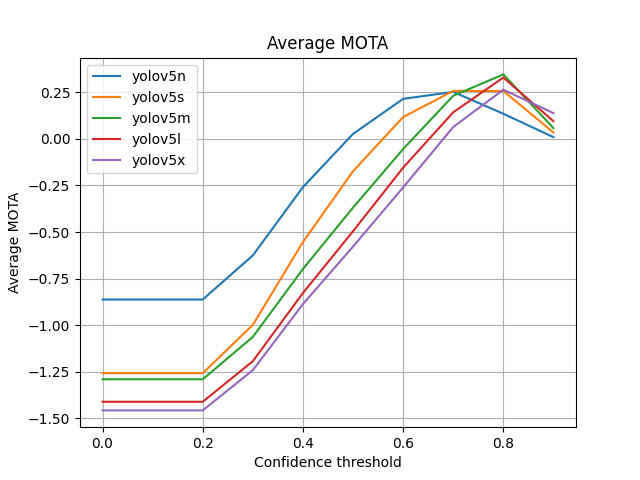
\includegraphics[width=0.49\textwidth]{figures/yolo_mota.png}
    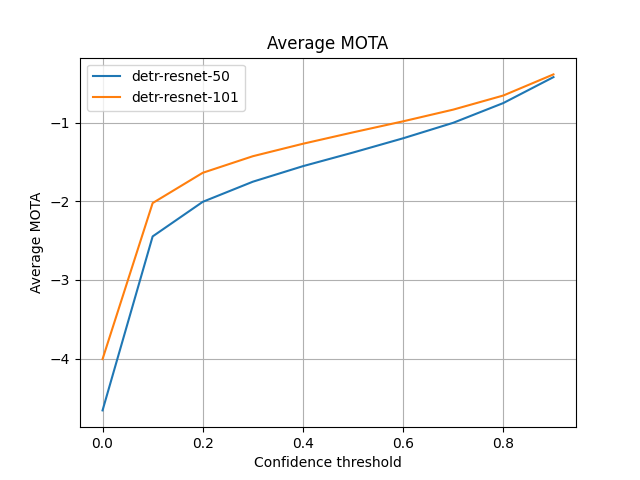
\includegraphics[width=0.49\textwidth]{figures/detr_mota.png}
    \caption{Average MOTA scores for each model.}
    \label{fig:avg-mota}
\end{figure}

\begin{figure}[h]
    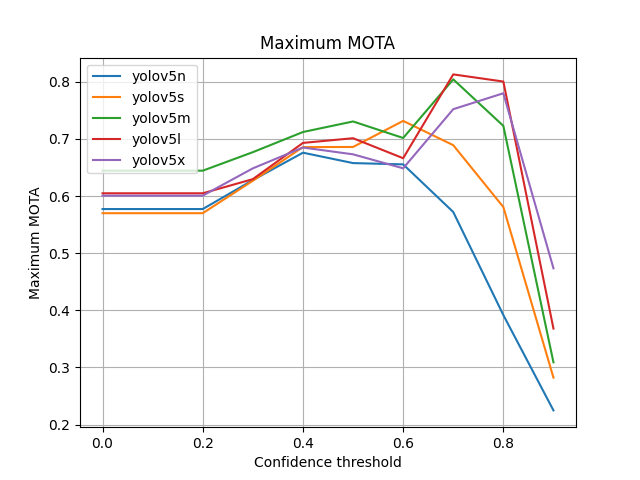
\includegraphics[width=0.49\textwidth]{figures/yolo_max_mota.png}
    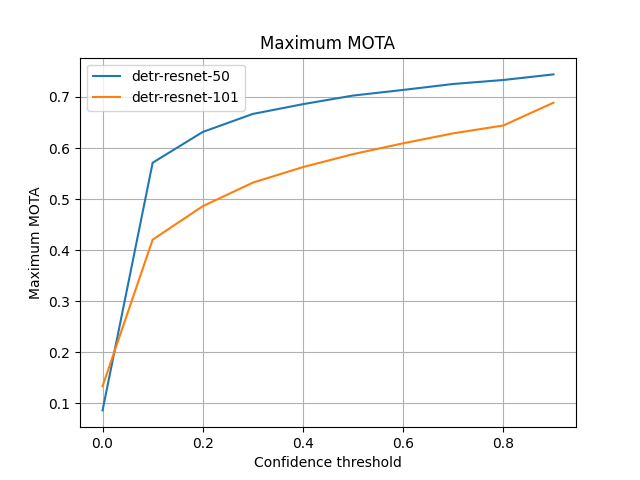
\includegraphics[width=0.49\textwidth]{figures/detr_max_mota.png}
    \caption{Maximum MOTA scores for each model.}
    \label{fig:max-mota}
\end{figure}

\subsection{Calculting benchmark scores}

Finally, I calculated the PR-MOTA score for each detector by joining the previous results along confidence thresholds, using trapezoidal rule approximation to calculate the integral:

\[\int_{\mathcal{C}}{MOTA(\textbf{s})d\textbf{s}} \approx \sum_{t = 2}^{10}{|C_tC_{t-1}|}\frac{MOTA(C_{t-1}) + MOTA(C_t)}{2} \]

where $C_1$, $C_2$, ..., $C_{10}$ are subsequent points on the $\mathcal{C}$ precision-recall curve defined by confidence thresholds between $0$ and $1$ with increments of $0.1$, while $|C_tC_{t-1}|$ denotes the distance between the two points. In practice, for the $1.0$ threshold the detectors supplied no output, so I defined their precision as $1$ (no bad hits) the recall as $0$ (found no true positive), and the $MOTA$ as $0$, in the spirit of the definition of these metrics.

The code for this step can be found, as usual, in the thesis' repository\footnote{\url{https://github.com/peter-i-istvan/bsc-thesis} under \texttt{tracking/calculte\_pr\_mota.py}, and also \texttt{pr\_mota.csv} for CSV results.}. The results can be seen in table~\ref{tab:pr-mota}. They can be considered relatively poor, and indicate that in the bigger part of the $[0;1]$ confidence interval, average MOTA scores are negative. This should be no suprise, because usually one does not trust the detections with confidence below 50\% (I found this to be true empirically, while experimenting with `off-the-shelf' pretrained models like these). The DETR underperforms the YOLO on this metric by a relatively large margin.

\begin{table}[h]
    \centering
    \begin{tabular}{|c|c|c|c|c|c|c|c|}
        \hline
        & D101 & D50 & YL& YM & YN & YS & YX \\
        \hline
        PR-MOTA & -1.33 & -1.51 & -0.42 & -0.37 & -0.19 & -0.33 & -0.46 \\
        \hline
    \end{tabular}
    \caption{PR-MOTA results.}
\label{tab:pr-mota}
\end{table}

The best among the DETR is the one with the ResNet101 backbone. This is not surprising, as the ResNet101 is the larger backbone, which usually means richer feature data to work with.  

Surprisingly, among the YOLO, the nano version had the best score. This was unexpected beacuse overall, the large and medium versions reached the highest scores. It can be somewhat explained looking at~\ref{fig:avg-mota}, where the nano version seems to have the highest signed area under the curve, and it has better performance on low confidence thresholds, but this only shows that the measurement is heavily influenced by how bad the tracking was at lower confidence. In production applications, one would chose a relatively high confidence threshold to start with, so the PR-MOTA score fails to predict future performance in such cases, as here the performance metrics on reasonable confidence thresholds are outweighted during averaging.



\section{Conclusion}

When viewing the final results by my chosen metric, the PR-MOTA score seems poor across all detectors. However, I concluded that, in this case, it is a flaw of the metric itself, which fails to predict usefulness in real life scenarios. As I observed, all the detectors I have tried give useless predictions under the confidence threshold of 50-60\% from the perspective of the SORT tracker. The measure of uselessness is almost irrelevant, but this difference is what caused the YOLOv5 nano to reach best score.

The real best performing object detectors were the YOLOv5 medium and large models, reaching about 35\% average MOTA on reasonable, 70-80\% confidence thresholds (in addition, the MOTA results obtained here show high variance, because even considering the average of 35\%, on some sequences it varies from -90\% to +80\% - see appendix). This is actually on par with SORT performance as first published in 2016~\cite{Bewley_2016} across various kinds of datasets, but considering the time passed since the publication, it would seem that the apparent improvement in detector quality in the meantime (from 2016 to 2020, publication date of the inspected models) has not brought great improvement in tracking performance. However, I suspect that this more related to the inspected detectors, and the way I evaluated them, than to the usefullness of SORT.

Both detectors were pretrained on the COCO 2017 dataset, a large and rich database of annotated images and numerous object classes, on a long and resource-hevy training regimen, the kind of which I could not replicate. Even though I only used three vehicle categories, the models themselves are capable of recognising much more, and during training the goal is to find all classes, and in all non-iconic poses too. Compared with the object feature distribution of the UA-DETRAC, COCO is richer both in number of object classes and in the context of the cars (the UA-DETRAC contains only vehicles engaged in road traffic, and from fixed camera angles). This generality of the COCO-trained models might hurt specific performance on UA-DETRAC, this is why fine-tuning on similar datasets, or even the vehicle subset of COCO would have helped. In this regard, considering the smaller visual diversity of UA-DETRAC, models from 2016 trained on it specifically can indeed perform on par with models from four years later, trained on COCO, even though the former models would score worse when trained on COCO, because of the inherent inferiority.

Regardless of the above, from the perspective of the original goal, the measurement provided insightful results in comparing a specific convolutional and and a specific Transformer-based object detector that were introduced roughly at the same time. Measurements from all aspects show that the COCO-trained YOLOv5 models outperform the COCO-trained DETR by a large margin when used in multiple vehicle tracking scenarios. It outperforms not only in quality, but in speed, as the inference and tracking times show that all versions of YOLOv5 are capable of real-time detection and tracking (when evaluated on my system), defined as 30 FPS or above, while the DETR versions are not, they are on average 3 to 6 times slower.

This concludes my inquiry, but it is needed to mention that from 2020 until the present, Transformer-based visual models, and object detectors specifically have seen great improvement, with introduction of new models like the Swin Transformer, Deformable DETR, Group DETR, GRiT, DINO etc. When inspecting leaderboards on Papers with Code\footnote{A popular online collection of machine learning publications, links to official codebases and benchmark results for comparison. See \url{https://paperswithcode.com/sota/object-detection-on-coco}}, it seems that evaluated on the COCO test set, the best of these currently outperform the YOLO series, but most convolutional object detectors as well. The only category where YOLO still has an edge is quality to speed ratio, as for real-time object detection, YOLOv7 is currently the leading model, outperforming fast visual Transformers like Swin.\footnote{\url{https://paperswithcode.com/sota/real-time-object-detection-on-coco}}.

% \include{content/transformer.tex}
% \chapter{Methods for transfer learning}

As I want to test both architectures' performance on a higher-order task (i.e. Multi Object Tracking), it is strongly advisable to train them for my specific workload. All the referenced neural network architectures have been trained on the COCO dataset, which is a large and diverse dataset of labeled images, containing X categories for `stuff` and Y categories for things. The capacity to distinguish between these can sometimes hurt the capacity to distinguish between a fewer number of categories. 


% %----------------------------------------------------------------------------
\chapter{\LaTeX-eszközök}
\label{sec:LatexTools}
%----------------------------------------------------------------------------
\section{A szerkesztéshez használatos eszközök}
%----------------------------------------------------------------------------
Ez a sablon TeXstudio 2.8.8 szerkesztővel készült. A TeXstudio egy platformfüggetlen, Windows, Linux és Mac OS alatt is elérhető \LaTeX-szerkesztőprogram számtalan hasznos szolgáltatással (\refstruc{fig:TeXstudio}). A szoftver ingyenesen letölthető\footnote{A TeXstudio hivatalos oldala: \url{http://texstudio.sourceforge.net/}}.

\begin{figure}[!ht]
\centering
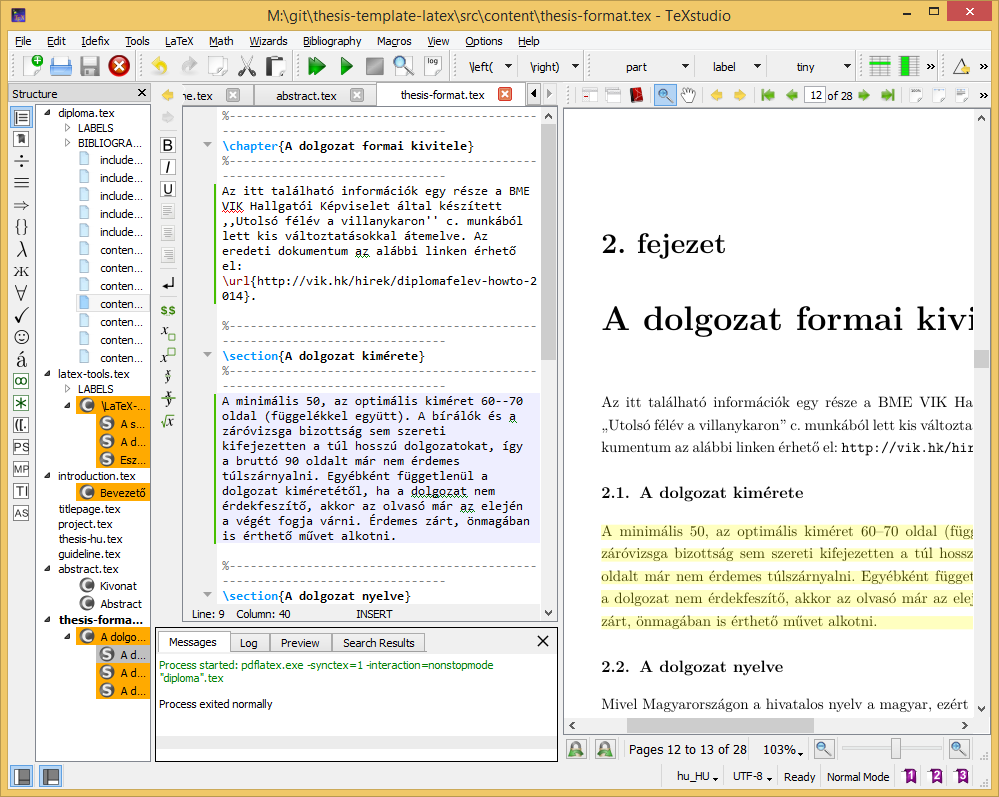
\includegraphics[width=150mm, keepaspectratio]{figures/TeXstudio.png}
\caption{A TeXstudio \LaTeX-szerkesztő.}
\label{fig:TeXstudio}
\end{figure}

A TeXstudio telepítése után érdemes még letölteni a magyar nyelvű helyesírásellenőrző-szótárakat hozzá. A TeXstudio az OpenOffice-hoz használatos formátumot tudja kezelni. A TeXstudio beállításainál a \verb+General+ fülön a \verb+Dictionaries+ résznél tudjuk megadni, hogy melyik szótárat használja.

Egy másik használható Windows alapú szerkesztőprogram a LEd\footnote{A LEd hivatalos oldala: \url{http://www.latexeditor.org/}} (LaTeX Editor), a TeXstudio azonban stabilabb, gyorsabb, és jobban használható.

%----------------------------------------------------------------------------
\section{A dokumentum lefordítása Windows alatt}
%----------------------------------------------------------------------------
A TeXstudio és a LEd kizárólag szerkesztőprogram (bár az utóbbiban DVI-nézegető is van), így a dokumentum fordításához szükséges eszközöket nem tartalmazza. Windows alatt alapvetően két lehetőség közül érdemes választani: MiKTeX (\url{http://miktex.org/}) és TeX Live (\url{http://www.tug.org/texlive/}) programcsomag. Az utóbbi működik Mac OS X, GNU/Linux alatt és Unix-származékokon is. A MiKTeX egy alapcsomag telepítése után mindig letölti a használt funkciókhoz szükséges, de lokálisan hiányzó \TeX-csomagokat, míg a TeX Live DVD ISO verzóban férhető hozzá. Ez a dokumentum TeX Live 2008 programcsomag segítségével fordult, amelynek DVD ISO verziója a megadott oldalról letölthető. A sablon lefordításához a disztribúcióban szereplő \verb+magyar.ldf+ fájlt a \verb+http://www.math.bme.hu/latex/+ változatra kell cserélni, vagy az utóbbi változatot be kell másolni a projekt-könyvtárba (ahogy ezt meg is tettük a sablonban) különben anomáliák tapasztalhatók a dokumentumban (pl. az ábra- és táblázat-aláírások formátuma nem a beállított lesz, vagy bizonyos oldalakon megjelenik alapértelmezésben egy fejléc). A TeX Live 2008-at még nem kell külön telepíteni a gépre, elegendő DVD-ről (vagy az ISO fájlból közvetlenül, pl. DaemonTools-szal) használni.

Ha a MiKTeX csomagot használjuk, akkor parancssorból a következő módon tudjuk újrafordítani a teljes dokumentumot:

\begin{lstlisting}[language=bash,frame=single,float=!ht]
$ texify -p thesis.tex
\end{lstlisting}

A \verb+texify+ parancs a MiKTex programcsomag \verb+miktex/bin+ alkönyvtárában található. A parancs gondoskodik arról, hogy a szükséges lépéseket (fordítás, hivatkozások generálása stb.) a megfelelő sorrendben elvégezze. A \verb+-p+ kapcsoló hatására PDF-et generál. A fordítást és az ideiglenes fájlok törlését elvégezhetjük a sablonhoz mellékelt \verb+manual_build.bat+ szkript segítségével is.

A \TeX-eszközöket tartalmazó programcsomag binárisainak elérési útját gyakran be kell állítani a szerkesztőprogramban, például TeXstudio esetén legegyszerűbben az \verb+Options / Configure TeXstudio... / Commands+ menüponttal előhívott dialógusablakban tehetjük ezt meg.

A PDF-\LaTeX~használata esetén a generált dokumentum közvetlenül PDF-formátumban áll rendelkezésre. Amennyiben a PDF-fájl egy PDF-nézőben (pl. Adobe Acrobat Reader vagy Foxit PDF Reader) meg van nyitva, akkor a fájlleírót a PDF-néző program tipikusan lefoglalja. Ilyen esetben a dokumentum újrafordítása hibaüzenettel kilép. Ha bezárjuk és újra megnyitjuk a PDF dokumentumot, akkor pedig a PDF-nézők többsége az első oldalon nyitja meg a dokumentumot, nem a legutóbb olvasott oldalon. Ezzel szemben például az egyszerű és ingyenes \textcolor{blue}{Sumatra PDF} nevű program képes arra, hogy a megnyitott dokumentum megváltozását detektálja, és frissítse a nézetet az aktuális oldal megtartásával.

%----------------------------------------------------------------------------
\section{Eszközök Linuxhoz}
%----------------------------------------------------------------------------
Linux operációs rendszer alatt is rengeteg szerkesztőprogram van, pl. a KDE alapú Kile jól használható. Ez ingyenesen letölthető, vagy éppenséggel az adott Linux-disztribúció eleve tartalmazza, ahogyan a dokumentum fordításához szükséges csomagokat is. Az Ubuntu Linux disztribúciók alatt például legtöbbször a \verb+texlive-*+ csomagok telepítésével használhatók a \LaTeX-eszközök. A jelen sablon fordításához szükséges csomagok (kb. 0,5 GB) az alábbi paranccsal telepíthetők:

\begin{lstlisting}[language=bash,morekeywords={sudo,apt\-get},alsoletter={-},breaklines=true]
$ sudo apt-get install texlive-latex-extra texlive-fonts-extra texlive-fonts-recommended texlive-xetex texlive-science
\end{lstlisting}

Amennyiben egy újabb csomag hozzáadása után hiányzó fájlra utaló hibát kapunk a fordítótól, telepítenünk kell az azt tartalmazó TeX Live csomagot. Ha pl. a \verb+bibentry+ csomagot szeretnénk használni, futtassuk az alábbi parancsot:

\begin{lstlisting}[language=bash,morekeywords={apt\-cache},alsoletter={-},breaklines=true]
$ apt-cache search bibentry
texlive-luatex - TeX Live: LuaTeX packages
\end{lstlisting}

Majd telepítsük fel a megfelelő TeX Live csomagot, jelen esetben a `texlive-lualatex`-et. (Egy LaTeX csomag több TeX Live csomagban is szerepelhet.)

Ha gyakran szerkesztünk más \LaTeX dokumentumokat is, kényelmes és biztos megoldás a teljes TeX Live disztribúció telepítése, ez azonban kb. 4 GB helyet igényel.

\begin{lstlisting}[language=bash,morekeywords={sudo,apt\-get},alsoletter={-},breaklines=true]
sudo apt-get install texlive-full
\end{lstlisting}

% %----------------------------------------------------------------------------
\chapter{A dolgozat formai kivitele}
%----------------------------------------------------------------------------
Az itt található információk egy része a BME VIK Hallgatói Képviselet által készített ,,Utolsó félév a villanykaron'' c. munkából lett kis változtatásokkal átemelve. Az eredeti dokumentum az alábbi linken érhető el: \url{http://vik.hk/hirek/diplomafelev-howto-2015}.

%----------------------------------------------------------------------------
\section{A dolgozat kimérete}
%----------------------------------------------------------------------------
Szakdolgozat esetében minimum 30, 45 körüli ajánlott oldalszám lehet az iránymutató. De mindenképp érdemes rákérdezni a konzulensnél is az elvárásokra, mert tanszékenként változóak lehetnek az elvárások.

Mesterképzésen a Diplomatervezés 1 esetében a beszámoló még inkább az Önálló laboratóriumi beszámolókhoz hasonlít, tanszékenként eltérő formai követelményekkel, -- egy legalább 30 oldal körüli dolgozat az elvárt -- és az elmúlt fél éves munkáról szól. De egyben célszerű, ha ez a végleges diplomaterv alapja is. (A végleges 60-90 oldal körülbelül a hasznos részre nézve)


%----------------------------------------------------------------------------
\section{A dolgozat nyelve}
%----------------------------------------------------------------------------
Mivel Magyarországon a hivatalos nyelv a magyar, ezért alapértelmezésben magyarul kell megírni a dolgozatot. Aki külföldi posztgraduális képzésben akar részt venni, nemzetközi szintű tudományos kutatást szeretne végezni, vagy multinacionális cégnél akar elhelyezkedni, annak célszerű angolul megírnia diplomadolgozatát. Mielőtt a hallgató az angol nyelvű verzió mellett dönt, erősen ajánlott mérlegelni, hogy ez mennyi többletmunkát fog a hallgatónak jelenteni fogalmazás és nyelvhelyesség terén, valamint -- nem utolsó sorban -- hogy ez mennyi többletmunkát fog jelenteni a konzulens illetve bíráló számára. Egy nehezen olvasható, netalán érthetetlen szöveg teher minden játékos számára.

%----------------------------------------------------------------------------
\section{A dokumentum nyomdatechnikai kivitele}
%----------------------------------------------------------------------------
A dolgozatot A4-es fehér lapra nyomtatva, 2,5 centiméteres margóval (+1~cm kötésbeni), 11--12 pontos betűmérettel, talpas betűtípussal és másfeles sorközzel célszerű elkészíteni.

Annak érdekében, hogy a dolgozat külsőleg is igényes munka benyomását keltse, érdemes figyelni az alapvető tipográfiai szabályok betartására~\cite{Jeney}.

% !TeX spellcheck = hu_HU
% !TeX encoding = UTF-8
% !TeX program = xelatex
%----------------------------------------------------------------------------
\chapter{A \LaTeX-sablon használata}
%----------------------------------------------------------------------------

Ebben a fejezetben röviden, implicit módon bemutatjuk a sablon használatának módját, ami azt jelenti, hogy sablon használata ennek a dokumentumnak a forráskódját tanulmányozva válik teljesen világossá. Amennyiben a szoftver-keretrendszer telepítve van, a sablon alkalmazása és a dolgozat szerkesztése \LaTeX-ben a sablon segítségével tapasztalataink szerint jóval hatékonyabb, mint egy WYSWYG (\emph{What You See is What You Get}) típusú szövegszerkesztő esetén (pl. Microsoft Word, OpenOffice).

%----------------------------------------------------------------------------
\section{Címkék és hivatkozások}
%----------------------------------------------------------------------------
A \LaTeX~dokumentumban címkéket (\verb+\label+) rendelhetünk ábrákhoz, táblázatokhoz, fejezetekhez, listákhoz, képletekhez stb. Ezekre a dokumentum bármely részében hivatkozhatunk, a hivatkozások automatikusan feloldásra kerülnek.

A sablonban makrókat definiáltunk a hivatkozások megkönnyítéséhez. Ennek megfelelően minden ábra (\emph{figure}) címkéje \verb+fig:+ kulcsszóval kezdődik, míg minden táblázat (\emph{table}), képlet (\emph{equation}), fejezet (\emph{section}) és lista (\emph{listing}) rendre a \verb+tab:+, \verb+eq:+, \verb+sec:+ és \verb+lst:+ kulcsszóval kezdődik, és a kulcsszavak után tetszőlegesen választott címke használható. Ha ezt a konvenciót betartjuk, akkor az előbbi objektumok számára rendre a \verb+\figref+, \verb+\tabref+, \verb+\eqref+, \verb+\sectref+ és \verb+\listref+ makrókkal hivatkozhatunk. A makrók paramétere a címke, amelyre hivatkozunk (a kulcsszó nélkül). Az összes említett hivatkozástípus, beleértve az \verb+\url+ kulcsszóval bevezetett web-hivatkozásokat is a  \verb+hyperref+\footnote{Segítségével a dokumentumban megjelenő hivatkozások nem csak dinamikussá válnak, de színezhetők is, bővebbet erről a csomag dokumentációjában találunk. Ez egyúttal egy példa lábjegyzet írására.} csomagnak köszönhetően aktívak a legtöbb PDF-nézegetőben, rájuk kattintva a dokumentum megfelelő oldalára ugrik a PDF-néző vagy a megfelelő linket megnyitja az alapértelmezett böngészővel. A \verb+hyperref+ csomag a kimeneti PDF-dokumentumba könyvjelzőket is készít a tartalomjegyzékből. Ez egy szintén aktív tartalomjegyzék, amelynek elemeire kattintva a nézegető behozza a kiválasztott fejezetet.

%----------------------------------------------------------------------------
\section{Ábrák és táblázatok}
%----------------------------------------------------------------------------
Használjunk vektorgrafikus ábrákat, ha van rá módunk. PDFLaTeX használata esetén PDF formátumú ábrákat lehet beilleszteni könnyen, az EPS (PostScript) vektorgrafikus képformátum beillesztését a PDFLaTeX közvetlenül nem támogatja (de lehet konvertálni, lásd később). Ha vektorgrafikus formában nem áll rendelkezésünkre az ábra, akkor a  veszteségmentes PNG, valamint a veszteséges JPEG formátumban érdemes elmenteni.  Figyeljünk arra, hogy ilyenkor a képek felbontása elég nagy legyen ahhoz, hogy nyomtatásban is megfelelő minőséget nyújtson (legalább 300 dpi javasolt). A dokumentumban felhasznált képfájlokat a dokumentum forrása mellett érdemes tartani, archiválni, mivel ezek hiányában a dokumentum nem fordul újra. Ha lehet, a vektorgrafikus képeket vektorgrafikus formátumban is érdemes elmenteni az újrafelhasználhatóság (az átszerkeszthetőség) érdekében.

Kapcsolási rajzok legtöbbször kimásolhatók egy vektorgrafikus programba (pl. CorelDraw) és onnan nagyobb felbontással raszterizálva kimenthatők PNG formátumban. Ugyanakkor kiváló ábrák készíthetők Microsoft Visio vagy hasonló program használatával is: Visio-ból az ábrák közvetlenül PDF-be is menthetők.

Lehetőségeink Matlab ábrák esetén:
\begin{itemize}
	\item Képernyőlopás (\emph{screenshot}) is elfogadható minőségű lehet a dokumentumban, de általában jobb felbontást is el lehet érni más módszerrel.
	\item A Matlab ábrát a \verb+File/Save As+ opcióval lementhetjük PNG formátumban (ugyanaz itt is érvényes, mint korábban, ezért nem javasoljuk).
	\item A Matlab ábrát az \verb+Edit/Copy figure+ opcióval kimásolhatjuk egy vektorgrafikus programba is és onnan nagyobb felbontással raszterizálva kimenthatjük PNG formátumban (nem javasolt).
	\item Javasolt megoldás: az ábrát a \verb+File/Save As+ opcióval EPS \emph{vektorgrafikus} formátumban elmentjük, PDF-be konvertálva beillesztjük a dolgozatba.
\end{itemize}
Az EPS kép az \verb+epstopdf+ programmal\footnote{a korábban említett \LaTeX-disztribúciókban megtalálható} konvertálható PDF formátumba. Célszerű egy batch-fájlt készíteni az összes EPS ábra lefordítására az alábbi módon (ez Windows alatt működik).
\begin{lstlisting}[language=]
@echo off
for %%j in (*.eps) do (
  echo converting file "%%j"
  epstopdf "%%j"
)
echo done .
\end{lstlisting}

Egy ilyen parancsfájlt (\verb+convert.cmd+) elhelyeztük a sablon \verb+figures\eps+ könyvtárába, így a felhasználónak csak annyi a dolga, hogy a \verb+figures\eps+ könyvtárba kimenti az EPS formátumú vektorgrafikus képet, majd lefuttatja a \verb+convert.cmd+ parancsfájlt, ami PDF-be konvertálja az EPS fájlt.

Ezek után a PDF-ábrát ugyanúgy lehet a dokumentumba beilleszteni, mint a PNG-t vagy a JPEG-et. A megoldás előnye, hogy a lefordított dokumentumban is vektorgrafikusan tárolódik az ábra, így a mérete jóval kisebb, mintha raszterizáltuk volna beillesztés előtt. Ez a módszer minden -- az EPS formátumot ismerő -- vektorgrafikus program (pl. CorelDraw) esetén is használható.

A képek beillesztésére \az+\refstruc{sec:LatexTools}ben mutattunk be példát (\refstruc{fig:TeXstudio}). Az előző mondatban egyúttal az automatikusan feloldódó ábrahivatkozásra is láthatunk példát. Több képfájlt is beilleszthetünk egyetlen ábrába. Az egyes képek közötti horizontális és vertikális margót metrikusan szabályozhatjuk (\refstruc{fig:HVSpaces}). Az ábrák elhelyezését számtalan tipográfiai szabály egyidejű teljesítésével a fordító maga végzi, a dokumentum írója csak preferenciáit jelezheti a fordító felé (olykor ez bosszúságot is okozhat, ilyenkor pl. a kép méretével lehet játszani).

\begin{figure}[!ht]
	\centering
	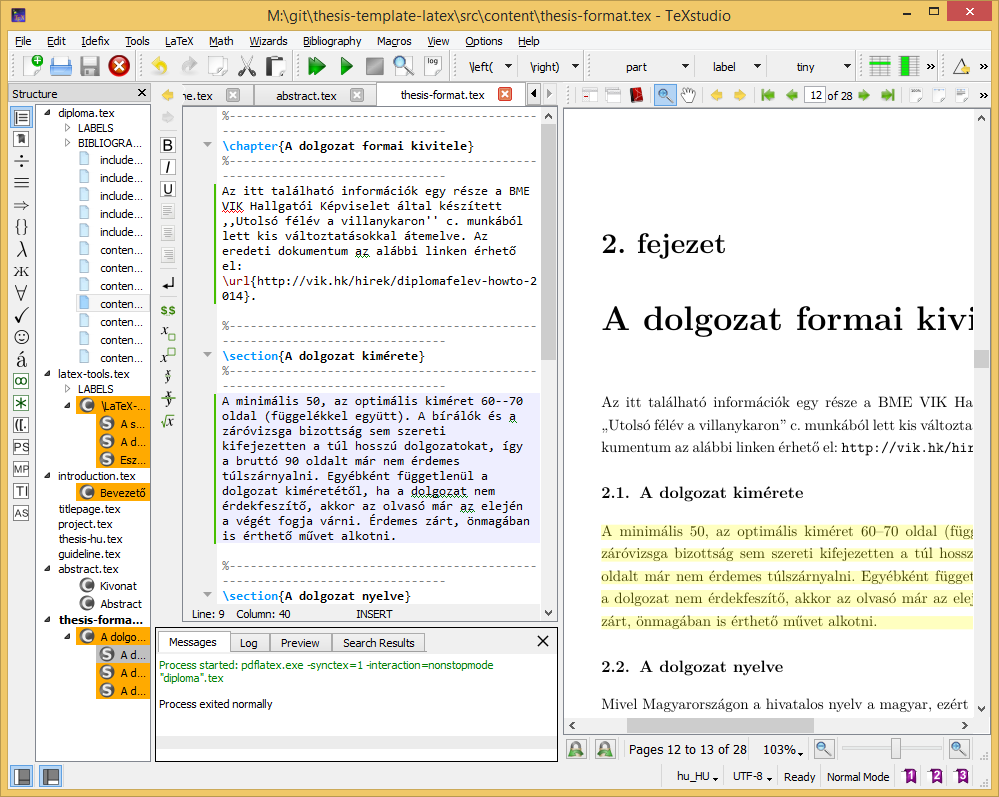
\includegraphics[width=67mm, keepaspectratio]{figures/TeXstudio.png}\hspace{1cm}
	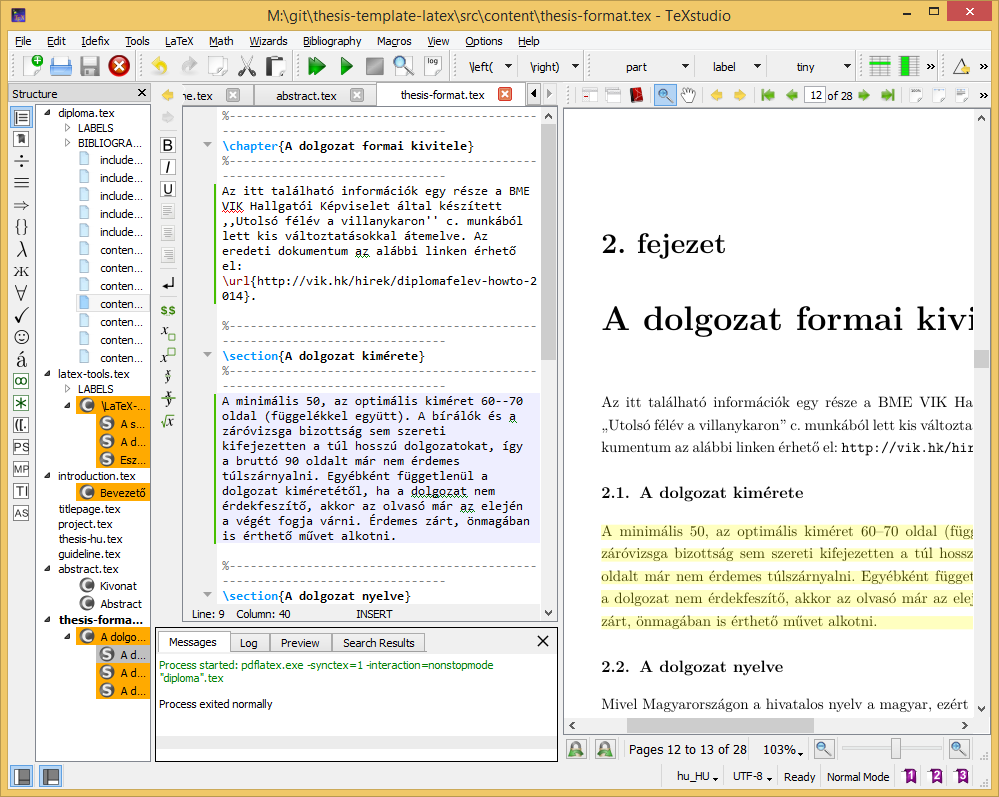
\includegraphics[width=67mm, keepaspectratio]{figures/TeXstudio.png}\\\vspace{5mm}
	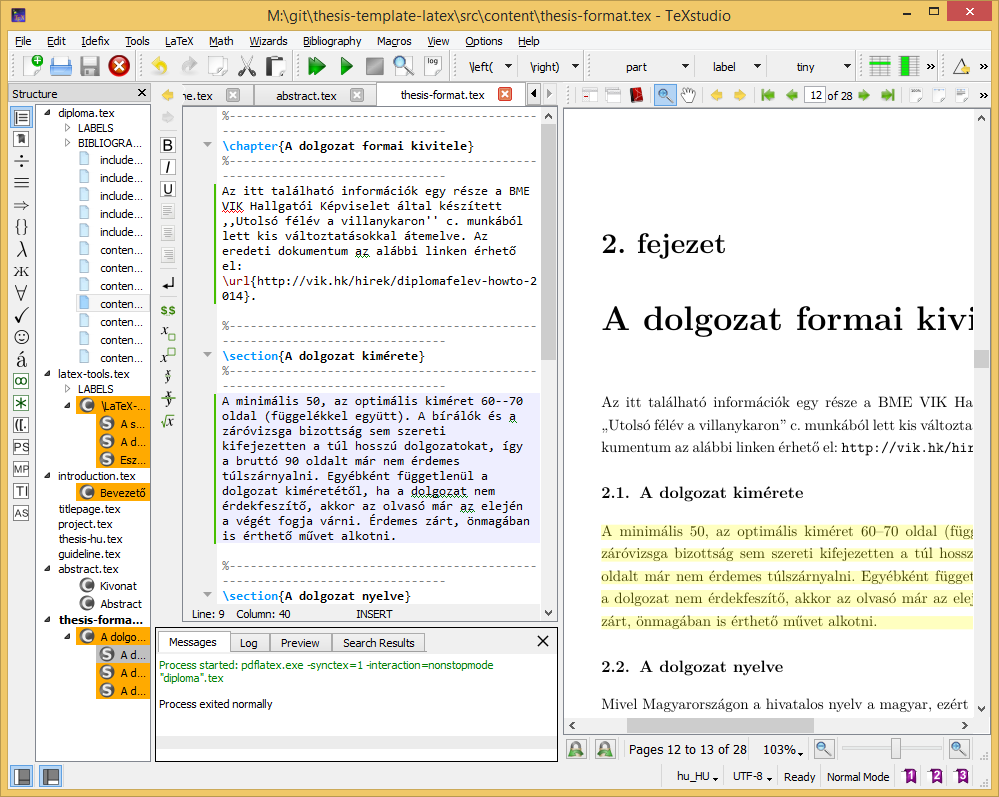
\includegraphics[width=67mm, keepaspectratio]{figures/TeXstudio.png}\hspace{1cm}
	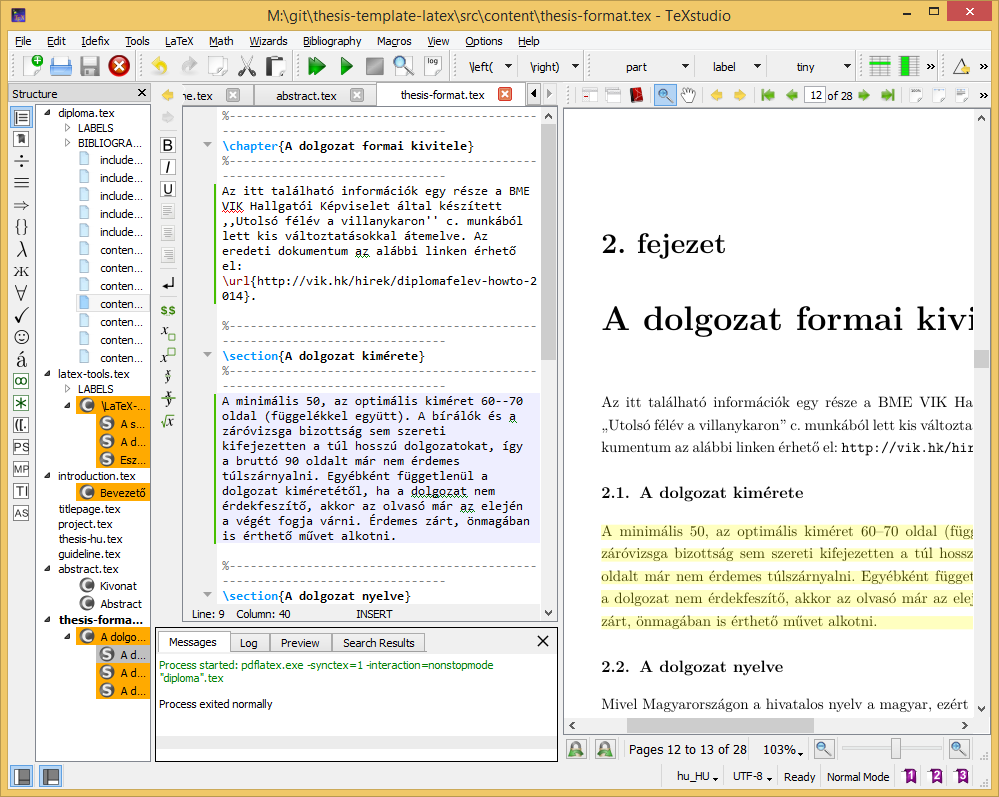
\includegraphics[width=67mm, keepaspectratio]{figures/TeXstudio.png}
	\caption{Több képfájl beillesztése esetén térközöket is érdemes használni.}
	\label{fig:HVSpaces}
\end{figure}

A táblázatok használatára \aref{tab:TabularExample}~táblázat mutat példát. A táblázatok formázásához hasznos tanácsokat találunk a \verb+booktabs+ csomag dokumentációjában.

\begin{table}[ht]
	\footnotesize
	\centering
	\begin{tabular}{ l c c }
		\toprule
		Órajel & Frekvencia & Cél pin \\
		\midrule
		CLKA & 100 MHz & FPGA CLK0\\
		CLKB & 48 MHz  & FPGA CLK1\\
		CLKC & 20 MHz  & Processzor\\
		CLKD & 25 MHz  & Ethernet chip \\
		CLKE & 72 MHz  & FPGA CLK2\\
		XBUF & 20 MHz  & FPGA CLK3\\
		\bottomrule
	\end{tabular}
	\caption{Az órajel-generátor chip órajel-kimenetei.}
	\label{tab:TabularExample}
\end{table}


%----------------------------------------------------------------------------
\section{Felsorolások és listák}
%----------------------------------------------------------------------------
Számozatlan felsorolásra mutat példát a jelenlegi bekezdés:
\begin{itemize}
	\item \emph{első bajusz:} ide lehetne írni az első elem kifejését,
	\item \emph{második bajusz:} ide lehetne írni a második elem kifejését,
	\item \emph{ez meg egy szakáll:} ide lehetne írni a harmadik elem kifejését.
\end{itemize}

Számozott felsorolást is készíthetünk az alábbi módon:
\begin{enumerate}
	\item \emph{első bajusz:} ide lehetne írni az első elem kifejését, és ez a kifejtés így néz ki, ha több sorosra sikeredik,
	\item \emph{második bajusz:} ide lehetne írni a második elem kifejését,
	\item \emph{ez meg egy szakáll:} ide lehetne írni a harmadik elem kifejését.
\end{enumerate}
A felsorolásokban sorok végén vessző, az utolsó sor végén pedig pont a szokásos írásjel. Ez alól kivételt képezhet, ha az egyes elemek több teljes mondatot tartalmaznak.

Listákban a dolgozat szövegétől elkülönítendő kódrészleteket, programsorokat, pszeudo-kódokat jeleníthetünk meg (\ref{lst:Example}.~kódrészlet).
\begin{lstlisting}[language=tex,caption=A fenti számozott felsorolás \LaTeX-forráskódja,label=lst:Example]
\begin{enumerate}
	\item \emph{els(*@ő@*) bajusz:} ide lehetne írni az els(*@ő@*) elem kifejését,
	és ez a kifejtés így néz ki, ha több sorosra sikeredik,
	\item \emph{második bajusz:} ide lehetne írni a második elem kifejését,
	\item \emph{ez meg egy szakáll:} ide lehetne írni a harmadik elem kifejését.
\end{enumerate}
\end{lstlisting}
A lista keretét, háttérszínét, egész stílusát megválaszthatjuk. Ráadásul különféle programnyelveket és a nyelveken belül kulcsszavakat is definiálhatunk, ha szükséges. Erről bővebbet a \verb+listings+ csomag hivatalos leírásában találhatunk.

%----------------------------------------------------------------------------
\section{Képletek}
%----------------------------------------------------------------------------
Ha egy formula nem túlságosan hosszú, és nem akarjuk hivatkozni a szövegből, mint például a $e^{i\pi}+1=0$ képlet, \emph{szövegközi képletként} szokás leírni. Csak, hogy másik példát is lássunk, az $U_i=-d\Phi/dt$ Faraday-törvény a $\rot E=-\frac{dB}{dt}$ differenciális alakban adott Maxwell-egyenlet felületre vett integráljából vezethető le. Látható, hogy a \LaTeX-fordító a sorközöket betartja, így a szöveg szedése esztétikus marad szövegközi képletek használata esetén is.

Képletek esetén az általános konvenció, hogy a kisbetűk skalárt, a kis félkövér betűk ($\mathbf{v}$) oszlopvektort -- és ennek megfelelően $\mathbf{v}^T$ sorvektort -- a kapitális félkövér betűk ($\mathbf{V}$) mátrixot jelölnek. Ha ettől el szeretnénk térni, akkor az alkalmazni kívánt jelölésmódot célszerű külön alfejezetben definiálni. Ennek megfelelően, amennyiben $\mathbf{y}$ jelöli a mérések vektorát, $\mathbf{\vartheta}$ a paraméterek vektorát és $\hat{\mathbf{y}}=\mathbf{X}\vartheta$ a paraméterekben lineáris modellt, akkor a \emph{Least-Squares} értelemben optimális paraméterbecslő $\hat{\mathbf{\vartheta}}_{LS}=(\mathbf{X}^T\mathbf{X})^{-1}\mathbf{X}^T\mathbf{y}$ lesz.

Emellett kiemelt, sorszámozott képleteket is megadhatunk, ennél az \verb+equation+ és a \verb+eqnarray+ környezetek helyett a korszerűbb \verb+align+ környezet alkalmazását javasoljuk (több okból, különféle problémák elkerülése végett, amelyekre most nem térünk ki). Tehát
\begin{align}
\dot{\mathbf{x}}&=\mathbf{A}\mathbf{x}+\mathbf{B}\mathbf{u},\\
\mathbf{y}&=\mathbf{C}\mathbf{x},
\end{align}
ahol $\mathbf{x}$ az állapotvektor, $\mathbf{y}$ a mérések vektora és $\mathbf{A}$, $\mathbf{B}$ és $\mathbf{C}$ a rendszert leíró paramétermátrixok. Figyeljük meg, hogy a két egyenletben az egyenlőségjelek egymáshoz igazítva jelennek meg, mivel a mindkettőt az \& karakter előzi meg a kódban. Lehetőség van számozatlan kiemelt képlet használatára is, például
\begin{align}
\dot{\mathbf{x}}&=\mathbf{A}\mathbf{x}+\mathbf{B}\mathbf{u},\nonumber\\
\mathbf{y}&=\mathbf{C}\mathbf{x}\nonumber.
\end{align}
Mátrixok felírására az $\mathbf{A}\mathbf{x}=\mathbf{b}$ inhomogén lineáris egyenlet részletes kifejtésével mutatunk példát:
\begin{align}
\begin{bmatrix}
a_{11} & a_{12} & \dots & a_{1n}\\
a_{21} & a_{22} & \dots & a_{2n}\\
\vdots & \vdots & \ddots & \vdots\\
a_{m1} & a_{m2} & \dots & a_{mn}
\end{bmatrix}
\begin{pmatrix}x_1\\x_2\\\vdots\\x_n\end{pmatrix}=
\begin{pmatrix}b_1\\b_2\\\vdots\\b_m\end{pmatrix}.
\end{align}
A \verb+\frac+ utasítás hatékonyságát egy általános másodfokú tag átviteli függvényén keresztül mutatjuk be, azaz
\begin{align}
W(s)=\frac{A}{1+2T\xi s+s^2T^2}.
\end{align}
A matematikai mód minden szimbólumának és képességének a bemutatására természetesen itt nincs lehetőség, de gyors referenciaként hatékonyan használhatók a következő linkek:\\
\indent\url{http://www.artofproblemsolving.com/LaTeX/AoPS_L_GuideSym.php},\\
\indent\url{http://www.ctan.org/tex-archive/info/symbols/comprehensive/symbols-a4.pdf},\\
\indent\url{ftp://ftp.ams.org/pub/tex/doc/amsmath/short-math-guide.pdf}.\\
Ez pedig itt egy magyarázat, hogy miért érdemes \verb+align+ környezetet használni:\\
\indent\url{http://texblog.net/latex-archive/maths/eqnarray-align-environment/}.

%----------------------------------------------------------------------------
\section{Irodalmi hivatkozások}
\label{sec:HowtoReference}
%----------------------------------------------------------------------------
Egy \LaTeX~dokumentumban az irodalmi hivatkozások definíciójának két módja van. Az egyik a \verb+\thebibliograhy+ környezet használata a dokumentum végén, az \verb+\end{document}+ lezárás előtt.
\begin{lstlisting}[language=tex]
\begin{thebibliography}{9}

\bibitem{Lamport94} Leslie Lamport, \emph{\LaTeX: A Document Preparation System}.
Addison Wesley, Massachusetts, 2nd Edition, 1994.

\end{thebibliography}
\end{lstlisting}

Ezek után a dokumentumban a \verb+\cite{Lamport94}+ utasítással hivatkozhatunk a forrásra. A fenti megadás viszonylag kötetlen, a szerző maga formázza az irodalomjegyzéket (ami gyakran inkonzisztens eredményhez vezet).

Egy sokkal professzionálisabb módszer a BiB\TeX{} használata, ezért ez a sablon is ezt támogatja. Ebben az esetben egy külön szöveges adatbázisban definiáljuk a forrásmunkákat, és egy külön stílusfájl határozza meg az irodalomjegyzék kinézetét. Ez, összhangban azzal, hogy külön formátumkonvenció határozza meg a folyóirat-, a könyv-, a konferenciacikk- stb. hivatkozások kinézetét az irodalomjegyzékben (a sablon használata esetén ezzel nem is kell foglalkoznia a hallgatónak, de az eredményt célszerű ellenőrizni). felhasznált hivatkozások adatbázisa egy \verb+.bib+ kiterjesztésű szöveges fájl, amelynek szerkezetét a \Aref{lst:Bibtex} kódrészlet demonstrálja. A forrásmunkák bevitelekor a sor végi vesszők külön figyelmet igényelnek, mert hiányuk a BiB\TeX-fordító hibaüzenetét eredményezi. A forrásmunkákat típus szerinti kulcsszó vezeti be (\verb+@book+ könyv, \verb+@inproceedings+ konferenciakiadványban megjelent cikk, \verb+@article+ folyóiratban megjelent cikk, \verb+@techreport+ valamelyik egyetem gondozásában megjelent műszaki tanulmány, \verb+@manual+ műszaki dokumentáció esetén stb.). Nemcsak a megjelenés stílusa, de a kötelezően megadandó mezők is típusról-típusra változnak. Egy jól használható referencia a \url{http://en.wikipedia.org/wiki/BibTeX} oldalon található.

\begin{lstlisting}[caption=Példa szöveges irodalomjegyzék-adatbázisra Bib\TeX{} használata esetén.,label=lst:Bibtex]
@book{Wettl04,
  author    = {Ferenc Wettl and Gyula Mayer and Péter Szabó},
  publisher = {Panem Könyvkiadó},
  title     = {\LaTeX~kézikönyv},
  year      = {2004},
}

@article{Candy86,
  author       = {James C. Candy},
  journaltitle = {{IEEE} Trans.\ on Communications},
  month        = {01},
  note         = {\doi{10.1109/TCOM.1986.1096432}},
  number       = {1},
  pages        = {72--76},
  title        = {Decimation for Sigma Delta Modulation},
  volume       = {34},
  year         = {1986},
}

@inproceedings{Lee87,
  author    = {Wai L. Lee and Charles G. Sodini},
  booktitle = {Proc.\ of the IEEE International Symposium on Circuits and Systems},
  location  = {Philadelphia, PA, USA},
  month     = {05~4--7},
  pages     = {459--462},
  title     = {A Topology for Higher Order Interpolative Coders},
  vol       = {2},
  year      = {1987},
}

@thesis{KissPhD,
  author      = {Peter Kiss},
  institution = {Technical University of Timi\c{s}oara, Romania},
  month       = {04},
  title       = {Adaptive Digital Compensation of Analog Circuit Imperfections for Cascaded Delta-Sigma Analog-to-Digital Converters},
  type        = {phdthesis},
  year        = {2000},
}

@manual{Schreier00,
  author       = {Richard Schreier},
  month        = {01},
  note         = {\url{http://www.mathworks.com/matlabcentral/fileexchange/}},
  organization = {Oregon State University},
  title        = {The Delta-Sigma Toolbox v5.2},
  year         = {2000},
}

@misc{DipPortal,
  author       = {{Budapesti Műszaki és Gazdaságtudományi Egyetem Villamosmérnöki és Informatikai Kar}},
  howpublished = {\url{http://diplomaterv.vik.bme.hu/}},
  title        = {Diplomaterv portál (2011. február 26.)},
}

@incollection{Mkrtychev:1997,
  author    = {Mkrtychev, Alexey},
  booktitle = {Logical Foundations of Computer Science},
  doi       = {10.1007/3-540-63045-7_27},
  editor    = {Adian, Sergei and Nerode, Anil},
  isbn      = {978-3-540-63045-6},
  pages     = {266-275},
  publisher = {Springer Berlin Heidelberg},
  series    = {Lecture Notes in Computer Science},
  title     = {Models for the logic of proofs},
  url       = {http://dx.doi.org/10.1007/3-540-63045-7_27},
  volume    = {1234},
  year      = {1997},
}
\end{lstlisting}

A stílusfájl egy \verb+.sty+ kiterjesztésű fájl, de ezzel lényegében nem kell foglalkozni, mert vannak beépített stílusok, amelyek jól használhatók. Ez a sablon a BiB\TeX-et használja, a hozzá tartozó adatbázisfájl a \verb+mybib.bib+ fájl. Megfigyelhető, hogy az irodalomjegyzéket a dokumentum végére (a \verb+\end{document}+ utasítás elé) beillesztett \verb+\bibliography{mybib}+ utasítással hozhatjuk létre, a stílusát pedig ugyanitt a  \verb+\bibliographystyle{plain}+ utasítással adhatjuk meg. Ebben az esetben a \verb+plain+ előre definiált stílust használjuk (a sablonban is ezt állítottuk be). A \verb+plain+ stíluson kívül természetesen számtalan más előre definiált stílus is létezik. Mivel a \verb+.bib+ adatbázisban ezeket megadtuk, a BiB\TeX-fordító is meg tudja különböztetni a szerzőt a címtől és a kiadótól, és ez alapján automatikusan generálódik az irodalomjegyzék a stílusfájl által meghatározott stílusban.

Az egyes forrásmunkákra a szövegből továbbra is a \verb+\cite+ paranccsal tudunk hivatkozni, így \aref{lst:Bibtex}.~kódrészlet esetén a hivatkozások rendre \verb+\cite{Wettl04}+, \verb+\cite{Candy86}+, \verb+\cite{Lee87}+, \verb+\cite{KissPhD}+, \verb+\cite{Schreirer00}+,
\verb+\cite{Mkrtychev:1997}+ és \verb+\cite{DipPortal}+. Az egyes forrásmunkák sorszáma az irodalomjegyzék bővítésekor változhat. Amennyiben az aktuális számhoz illeszkedő névelőt szeretnénk használni, használjuk az \verb+\acite{}+ parancsot.

Az irodalomjegyzékben alapértelmezésben csak azok a forrásmunkák jelennek meg, amelyekre található hivatkozás a szövegben, és ez így alapvetően helyes is, hiszen olyan forrásmunkákat nem illik az irodalomjegyzékbe írni, amelyekre nincs hivatkozás.

Mivel a fordítási folyamat során több lépésben oldódnak fel a szimbólumok, ezért gyakran többször is le kell fordítani a dokumentumot. Ilyenkor ez első 1-2 fordítás esetleg szimbólum-feloldásra vonatkozó figyelmeztető üzenettel zárul. Ha hibaüzenettel zárul bármelyik fordítás, akkor nincs értelme megismételni, hanem a hibát kell megkeresni. A \verb+.bib+ fájl megváltoztatáskor sokszor nincs hatása a változtatásnak azonnal, mivel nem mindig fut újra a BibTeX fordító. Ezért célszerű a változtatás után azt manuálisan is lefuttatni (TeXstudio esetén \verb+Tools/Bibliography+).

Hogy a szövegbe ágyazott hivatkozások kinézetét demonstráljuk, itt most sorban meghivatkozzuk a \cite{Wettl04}, \cite{Candy86}, \cite{Lee87}, \cite{KissPhD}, \cite{Schreier00} és \acite{Mkrtychev:1997}\footnote{Informatikai témában gyakran hivatkozunk cikkeket a Springer LNCS valamely kötetéből, ez a hivatkozás erre mutat egy helyes példát.} forrásmunkát, valamint \acite{DipPortal} weboldalt.

Megjegyzendő, hogy az ékezetes magyar betűket is tartalmazó \verb+.bib+ fájl az \verb+inputenc+ csomaggal betöltött \verb+latin2+ betűkészlet miatt fordítható. Ugyanez a \verb+.bib+ fájl hibaüzenettel fordul egy olyan dokumentumban, ami nem tartalmazza a \verb+\usepackage[latin2]{inputenc}+ sort. Speciális igény esetén az irodalmi adatbázis általánosabb érvényűvé tehető, ha az ékezetes betűket speciális latex karakterekkel helyettesítjük a \verb+.bib+ fájlban, pl. á helyett \verb+\'{a}+-t vagy ő helyett \verb+\H{o}+-t írunk.

Irodalomhivatkozásokat célszerű először olyan szolgáltatásokban keresni, ahol jó minőségű bejegyzések találhatók (pl. ACM Digital Library,\footnote{\url{https://dl.acm.org/}} DBLP,\footnote{\url{http://dblp.uni-trier.de/}} IEEE Xplore,\footnote{\url{http://ieeexplore.ieee.org/}} SpringerLink\footnote{\url{https://link.springer.com/}}) és csak ezek után használni kevésbé válogatott forrásokat (pl. Google Scholar\footnote{\url{http://scholar.google.com/}}). A jó minőségű bejegyzéseket is érdemes megfelelően tisztítani.\footnote{\url{https://github.com/FTSRG/cheat-sheets/wiki/BibTeX-Fixing-entries-from-common-sources}} A sablon angol nyelvű változatában használt \texttt{plainnat} beállítás egyik sajátossága, hogy a cikkhez generált hivatkozás a cikk DOI-ját és URL-jét is tartalmazza, ami gyakran duplikátumhoz vezet -- érdemes tehát a DOI-kat tartalmazó URL mezőket törölni. 

%----------------------------------------------------------------------------
\section{A dolgozat szerkezete és a forrásfájlok}
%----------------------------------------------------------------------------
A diplomatervsablonban a TeX fájlok két alkönyvtárban helyezkednek el. Az \verb+include+ könyvtárban azok szerepelnek, amiket tipikusan nem kell szerkesztenünk, ezek a sablon részei (pl. címoldal). A \verb+content+ alkönyvtárban pedig a saját munkánkat helyezhetjük el. Itt érdemes az egyes fejezeteket külön \TeX{} állományokba rakni.

A diplomatervsablon (a kari irányelvek szerint) az alábbi fő fejezetekből áll:
\begin{enumerate}
	\item 1 oldalas \emph{tájékoztató} a szakdolgozat/diplomaterv szerkezetéről (\verb+include/guideline.tex+), ami a végső dolgozatból törlendő,
	\item \emph{feladatkiírás} (\verb+include/project.tex+), a dolgozat nyomtatott verzójában ennek a helyére kerül a tanszék által kiadott, a tanszékvezető által aláírt feladatkiírás, a dolgozat elektronikus verziójába pedig a feladatkiírás egyáltalán ne kerüljön bele, azt külön tölti fel a tanszék a diplomaterv-honlapra,
	\item \emph{címoldal} (\verb+include/titlepage.tex+),
	\item \emph{tartalomjegyzék} (\verb+thesis.tex+),
	\item a diplomatervező \emph{nyilatkozat}a az önálló munkáról (\verb+include/declaration.tex+),
	\item 1-2 oldalas tartalmi \emph{összefoglaló} magyarul és angolul, illetve elkészíthető még további nyelveken is (\verb+content/abstract.tex+),
	\item \emph{bevezetés}: a feladat értelmezése, a tervezés célja, a feladat indokoltsága, a diplomaterv felépítésének rövid összefoglalása (\verb+content/introduction.tex+),
	\item sorszámmal ellátott \emph{fejezetek}: a feladatkiírás pontosítása és részletes elemzése, előzmények (irodalomkutatás, hasonló alkotások), az ezekből levonható következtetések, a tervezés részletes leírása, a döntési lehetőségek értékelése és a választott megoldások indoklása, a megtervezett műszaki alkotás értékelése, kritikai elemzése, továbbfejlesztési lehetőségek,
	\item esetleges \emph{köszönetnyilvánítás}ok (\verb+content/acknowledgement.tex+),
	\item részletes és pontos \emph{irodalomjegyzék} (ez a sablon esetében automatikusan generálódik a \verb+thesis.tex+ fájlban elhelyezett \verb+\bibliography+ utasítás hatására, \az+\refstruc{sec:HowtoReference}ban leírtak szerint),
	\item \emph{függelékek} (\verb+content/appendices.tex+).
\end{enumerate}

A sablonban a fejezetek a \verb+thesis.tex+ fájlba vannak beillesztve \verb+\include+ utasítások segítségével. Lehetőség van arra, hogy csak az éppen szerkesztés alatt álló \verb+.tex+ fájlt fordítsuk le, ezzel lerövidítve a fordítási folyamatot. Ezt a lehetőséget az alábbi kódrészlet biztosítja a \verb+thesis.tex+ fájlban.
\begin{lstlisting}
\includeonly{
	guideline,%
	project,%
	titlepage,%
	declaration,%
	abstract,%
	introduction,%
	chapter1,%
	chapter2,%
	chapter3,%
	acknowledgement,%
	appendices,%
}
\end{lstlisting}

Ha az alábbi kódrészletben az egyes sorokat a \verb+%+ szimbólummal kikommentezzük, akkor a megfelelő \verb+.tex+ fájl nem fordul le. Az oldalszámok és a tartalomjegyék természetesen csak akkor billennek helyre, ha a teljes dokumentumot lefordítjuk.

%----------------------------------------------------------------------------
\newpage
\section{Alapadatok megadása}
%----------------------------------------------------------------------------
A diplomaterv alapadatait (cím, szerző, konzulens, konzulens titulusa) a \verb+thesis.tex+ fájlban lehet megadni.

%----------------------------------------------------------------------------
\section{Új fejezet írása}
%----------------------------------------------------------------------------
A főfejezetek külön \verb+content+ könyvtárban foglalnak helyet. A sablonhoz 3 fejezet készült. További főfejezeteket úgy hozhatunk létre, ha új \TeX~fájlt készítünk a fejezet számára, és a \verb+thesis.tex+ fájlban, a \verb+\include+ és \verb+\includeonly+ utasítások argumentumába felvesszük az új \verb+.tex+ fájl nevét.


%----------------------------------------------------------------------------
\section{Definíciók, tételek, példák}
%----------------------------------------------------------------------------

\begin{definition}[Fluxuskondenzátor térerőssége]
Lorem ipsum dolor sit amet, consectetur adipiscing elit, sed do eiusmod tempor incididunt ut labore et dolore magna aliqua. Ut enim ad minim veniam, quis nostrud exercitation ullamco laboris nisi ut aliquip ex ea commodo consequat.
\end{definition}

\begin{example}
Példa egy példára. Duis aute irure dolor in reprehenderit in voluptate velit esse cillum dolore eu fugiat nulla pariatur. Excepteur sint occaecat cupidatat non proident, sunt in culpa qui officia deserunt mollit anim id est laborum.
\end{example}

\begin{theorem}[Kovács tétele]
Duis aute irure dolor in reprehenderit in voluptate velit esse cillum dolore eu fugiat nulla pariatur. Excepteur sint occaecat cupidatat non proident, sunt in culpa qui officia deserunt mollit anim id est laborum.
\end{theorem}



% Acknowledgements
%~~~~~~~~~~~~~~~~~~~~~~~~~~~~~~~~~~~~~~~~~~~~~~~~~~~~~~~~~~~~~~~~~~~~~~~~~~~~~~~~~~~~~~
% %----------------------------------------------------------------------------
\chapter*{\koszonetnyilvanitas}\addcontentsline{toc}{chapter}{\koszonetnyilvanitas}
%----------------------------------------------------------------------------

Ez nem kötelező, akár törölhető is. Ha a szerző szükségét érzi, itt lehet köszönetet nyilvánítani azoknak, akik hozzájárultak munkájukkal ahhoz, hogy a hallgató a szakdolgozatban vagy diplomamunkában leírt feladatokat sikeresen elvégezze. A konzulensnek való köszönetnyilvánítás sem kötelező, a konzulensnek hivatalosan is dolga, hogy a hallgatót konzultálja.


% List of Figures, Tables
%~~~~~~~~~~~~~~~~~~~~~~~~~~~~~~~~~~~~~~~~~~~~~~~~~~~~~~~~~~~~~~~~~~~~~~~~~~~~~~~~~~~~~~
%\listoffigures\addcontentsline{toc}{chapter}{\listfigurename}
%\listoftables\addcontentsline{toc}{chapter}{\listtablename}


% Bibliography
%~~~~~~~~~~~~~~~~~~~~~~~~~~~~~~~~~~~~~~~~~~~~~~~~~~~~~~~~~~~~~~~~~~~~~~~~~~~~~~~~~~~~~~
\addcontentsline{toc}{chapter}{\bibname}
\bibliography{bib/mybib}


% Appendix
%~~~~~~~~~~~~~~~~~~~~~~~~~~~~~~~~~~~~~~~~~~~~~~~~~~~~~~~~~~~~~~~~~~~~~~~~~~~~~~~~~~~~~~
% \clearpage
%----------------------------------------------------------------------------
\appendix
%----------------------------------------------------------------------------
\chapter*{\fuggelek}\addcontentsline{toc}{chapter}{\fuggelek}
\setcounter{chapter}{\appendixnumber}
%\setcounter{equation}{0} % a fofejezet-szamlalo az angol ABC 6. betuje (F) lesz
\numberwithin{equation}{section}
\numberwithin{figure}{section}
\numberwithin{lstlisting}{section}
%\numberwithin{tabular}{section}


\section{Precision-recall curves and tracking performances}

\begin{figure}[h]
    \captionsetup{width=\textwidth}
    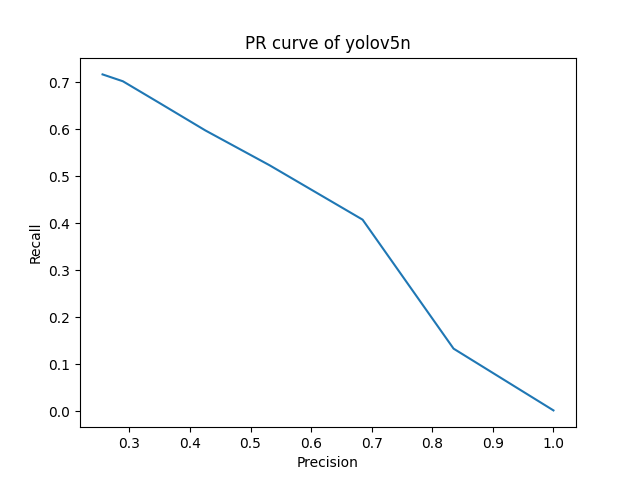
\includegraphics[width=0.49\textwidth]{figures/yolov5n.png}
    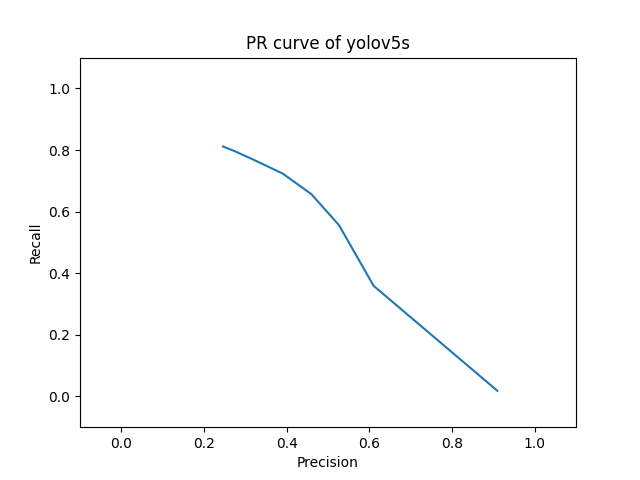
\includegraphics[width=0.49\textwidth]{figures/yolov5s.png} \\
    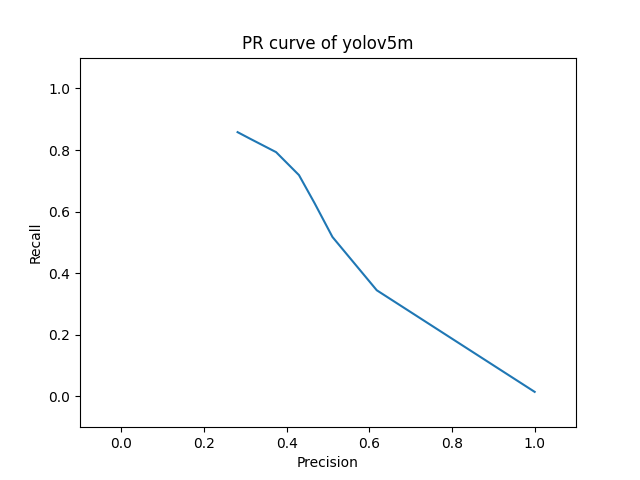
\includegraphics[width=0.49\textwidth]{figures/yolov5m.png}
    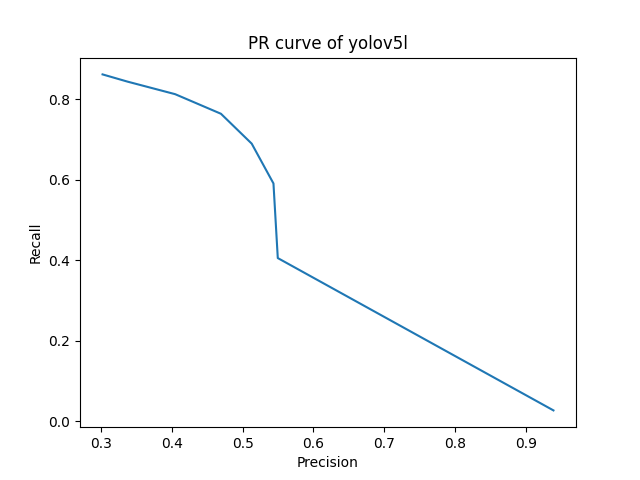
\includegraphics[width=0.49\textwidth]{figures/yolov5l.png} \\
    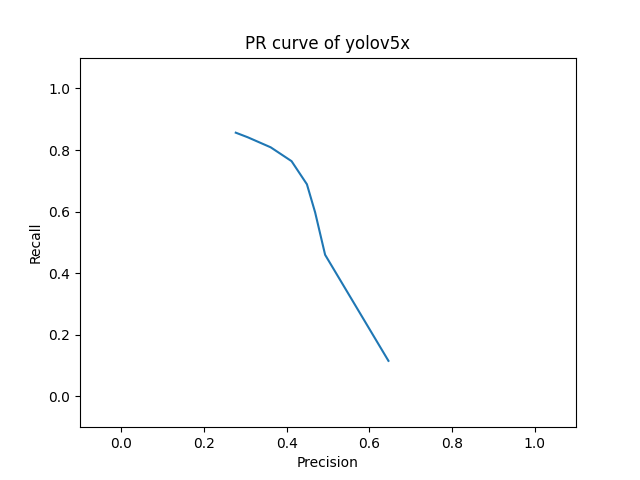
\includegraphics[width=0.49\textwidth]{figures/yolov5x.png}
    \caption{The PR curves of the five YOLO models.}
    \label{fig:pr_yolo}
\end{figure}

\clearpage

\begin{figure}[h]
    \captionsetup{width=\textwidth}
    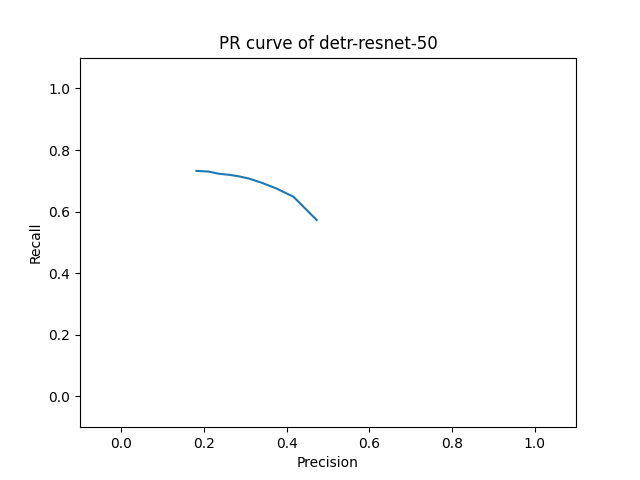
\includegraphics[width=0.49\textwidth]{figures/detr-resnet-50.png}
    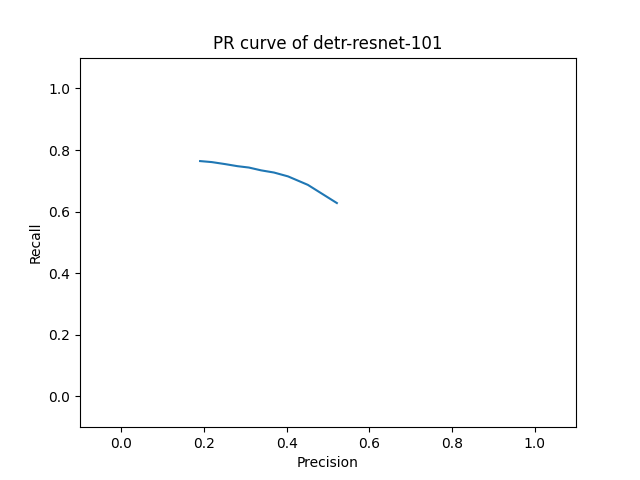
\includegraphics[width=0.49\textwidth]{figures/detr-resnet-101.png}
    \caption{The PR curves of the two DETR models.}
    \label{fig:pr_detr}
\end{figure}


% YN
\begin{table}[h]
    \centering
    \begin{tabular}{|c||c|c|c|c|c|c|c|c|}
        \hline
        CT & MOTA & MOTA\_m & MOTA\_M & MOTP & MT & ML & UO & IDS \\
        \hline
        \hline
        0.9 & 0.01 & 0.00 & 0.22 & nan & 1 & 5886 & 5936 & 43 \\
        \hline
        0.8 & 0.13 & -0.00 & 0.39 & 0.13 & 72 & 4411 & 5936 & 1017 \\
        \hline 
        0.7 & 0.25 & -0.46 & 0.57 & 0.14 & 520 & 2398 & 5936 & 1976 \\
        \hline 
        0.6 & 0.21 & -1.30 & 0.66 & 0.15 & 1143 & 1587 & 5936 & 1709 \\
        \hline 
        0.5 & 0.03 & -4.43 & 0.66 & 0.16 & 1702 & 1208 & 5936 & 1461 \\
        \hline 
        0.4 & -0.26 & -9.61 & 0.68 & 0.16 & 2227 & 1010 & 5936 & 1951 \\
        \hline 
        0.3 & -0.63 & -14.93 & 0.63 & 0.16 & 2583 & 903 & 5936 & 2969 \\
        \hline 
        0.2 & -0.86 & -17.49 & 0.58 & 0.16 & 2717 & 851 & 5936 & 3457 \\
        \hline 
        0.1 & -0.86 & -17.49 & 0.58 & 0.16 & 2717 & 851 & 5936 & 3457 \\
        \hline 
        0.0 & -0.86 & -17.49 & 0.58 & 0.16 & 2717 & 851 & 5936 & 3457 \\
        \hline
    \end{tabular}
    \caption{The performance metrics of the \textbf{YOLOv5 nano}, aggregated across all sequences. CT is the confidence threshold, MOTA is the average MOTA across all sequences, MOTA\_m is the minimum, while MOTA\_M is the maximum achieved on a sequence, MT is the number of mostly tracked trajectories, ML is the number of mostly lost trajectories (it is worth inspecting these in relation with UO - the number of unique object trajectories across all sequences), and IDS is the number of identity switches.}
    \label{tab:mota_yn}
\end{table}
% YS
\begin{table}[h]
    \centering
    \begin{tabular}{|c||c|c|c|c|c|c|c|c|}
        \hline
        CT & MOTA & MOTA\_m & MOTA\_M & MOTP & MT & ML & UO & IDS \\
        \hline
        \hline
        0.9 & 0.03 & 0.00 & 0.28 & nan & 5 & 5705 & 5936 & 248 \\
        \hline
        0.8 & 0.26 & -0.29 & 0.58 & 0.13 & 425 & 2758 & 5936 & 2159 \\
        \hline 
        0.7 & 0.26 & -1.45 & 0.69 & 0.14 & 1343 & 1468 & 5936 & 2087 \\
        \hline 
        0.6 & 0.12 & -2.26 & 0.73 & 0.15 & 2096 & 910 & 5936 & 1673 \\
        \hline 
        0.5 & -0.17 & -6.60 & 0.69 & 0.15 & 2743 & 645 & 5936 & 1819 \\
        \hline 
        0.4 & -0.55 & -12.92 & 0.69 & 0.15 & 3276 & 547 & 5936 & 2981 \\
        \hline 
        0.3 & -1.00 & -19.46 & 0.63 & 0.15 & 3575 & 487 & 5936 & 3934 \\
        \hline 
        0.2 & -1.26 & -22.12 & 0.57 & 0.15 & 3657 & 472 & 5936 & 4181 \\
        \hline 
        0.1 & -1.26 & -22.12 & 0.57 & 0.15 & 3657 & 472 & 5936 & 4181 \\
        \hline 
        0.0 & -1.26 & -22.12 & 0.57 & 0.15 & 3657 & 472 & 5936 & 4181 \\
        \hline 
    \end{tabular}
    \caption{The performance metrics of the \textbf{YOLOv5 small}, aggregated across all sequences. CT is the confidence threshold, MOTA is the average MOTA across all sequences, MOTA\_m is the minimum, while MOTA\_M is the maximum achieved on a sequence, MT is the number of mostly tracked trajectories, ML is the number of mostly lost trajectories (it is worth inspecting these in relation with UO - the number of unique object trajectories across all sequences), and IDS is the number of identity switches.}
    \label{tab:mota_ys}
\end{table}
% YM
\begin{table}[h]
    \centering
    \begin{tabular}{|c||c|c|c|c|c|c|c|c|}
        \hline
        CT & MOTA & MOTA\_m & MOTA\_M & MOTP & MT & ML & UO & IDS \\
        \hline
        \hline
        0.9 & 0.06 & 0.00 & 0.31 & nan & 9 & 5410 & 5936 & 354 \\
        \hline
        0.8 & 0.35 & -0.31 & 0.72 & 0.13 & 1019 & 1573 & 5936 & 1303 \\
        \hline 
        0.7 & 0.23 & -1.89 & 0.80 & 0.14 & 1874 & 917 & 5936 & 1192 \\
        \hline 
        0.6 & -0.05 & -6.69 & 0.70 & 0.14 & 2512 & 618 & 5936 & 1123 \\
        \hline 
        0.5 & -0.37 & -11.63 & 0.73 & 0.15 & 3095 & 505 & 5936 & 1332 \\
        \hline 
        0.4 & -0.70 & -15.28 & 0.71 & 0.15 & 3520 & 445 & 5936 & 1855 \\
        \hline 
        0.3 & -1.06 & -18.25 & 0.68 & 0.15 & 3803 & 407 & 5936 & 2138 \\
        \hline 
        0.2 & -1.29 & -20.29 & 0.64 & 0.15 & 3903 & 402 & 5936 & 2250 \\
        \hline 
        0.1 & -1.29 & -20.29 & 0.64 & 0.15 & 3903 & 402 & 5936 & 2250 \\
        \hline 
        0.0 & -1.29 & -20.29 & 0.64 & 0.15 & 3903 & 402 & 5936 & 2250 \\
        \hline
    \end{tabular}
    \caption{The performance metrics of the \textbf{YOLOv5 medium}, aggregated across all sequences. CT is the confidence threshold, MOTA is the average MOTA across all sequences, MOTA\_m is the minimum, while MOTA\_M is the maximum achieved on a sequence, MT is the number of mostly tracked trajectories, ML is the number of mostly lost trajectories (it is worth inspecting these in relation with UO - the number of unique object trajectories across all sequences), and IDS is the number of identity switches.}
    \label{tab:mota_ym}
\end{table}
% YL
\begin{table}[h]
    \centering
    \begin{tabular}{|c||c|c|c|c|c|c|c|c|}
        \hline
        CT & MOTA & MOTA\_m & MOTA\_M & MOTP & MT & ML & UO & IDS \\
        \hline
        \hline
        0.9 & 0.09 & 0.00 & 0.37 & 0.11 & 27 & 4986 & 5936 & 464 \\
        \hline
        0.8 & 0.33 & -0.97 & 0.80 & 0.14 & 1363 & 1459 & 5936 & 1542 \\
        \hline
        0.7 & 0.14 & -2.68 & 0.81 & 0.14 & 2317 & 850 & 5936 & 1269 \\
        \hline
        0.6 & -0.15 & -6.70 & 0.67 & 0.15 & 2880 & 587 & 5936 & 1171 \\
        \hline
        0.5 & -0.50 & -12.43 & 0.70 & 0.15 & 3341 & 460 & 5936 & 1214 \\
        \hline
        0.4 & -0.83 & -16.11 & 0.69 & 0.15 & 3692 & 403 & 5936 & 1863 \\
        \hline
        0.3 & -1.19 & -18.49 & 0.63 & 0.15 & 3899 & 372 & 5936 & 2120 \\
        \hline
        0.2 & -1.41 & -19.76 & 0.60 & 0.15 & 3956 & 371 & 5936 & 2197 \\
        \hline
        0.1 & -1.41 & -19.76 & 0.60 & 0.15 & 3956 & 371 & 5936 & 2197 \\
        \hline
        0.0 & -1.41 & -19.76 & 0.60 & 0.15 & 3956 & 371 & 5936 & 2197 \\
        \hline
    \end{tabular}
    \caption{The performance metrics of the \textbf{YOLOv5 large}, aggregated across all sequences. CT is the confidence threshold, MOTA is the average MOTA across all sequences, MOTA\_m is the minimum, while MOTA\_M is the maximum achieved on a sequence, MT is the number of mostly tracked trajectories, ML is the number of mostly lost trajectories (it is worth inspecting these in relation with UO - the number of unique object trajectories across all sequences), and IDS is the number of identity switches.}
    \label{tab:mota_yl}
\end{table}
% YX
\begin{table}[h]
    \centering
    \begin{tabular}{|c||c|c|c|c|c|c|c|c|}
        \hline
        CT & MOTA & MOTA\_m & MOTA\_M & MOTP & MT & ML & UO & IDS \\
        \hline
        \hline
        0.9 & 0.14 & -0.17 & 0.47 & 0.11 & 72 & 4455 & 5936 & 633 \\
        \hline
        0.8 & 0.26 & -2.46 & 0.78 & 0.13 & 1323 & 1529 & 5936 & 1204 \\
        \hline
        0.7 & 0.06 & -3.48 & 0.75 & 0.14 & 2079 & 908 & 5936 & 1254 \\
        \hline
        0.6 & -0.26 & -8.14 & 0.65 & 0.14 & 2663 & 596 & 5936 & 1152 \\
        \hline
        0.5 & -0.58 & -13.07 & 0.67 & 0.15 & 3213 & 457 & 5936 & 1483 \\
        \hline
        0.4 & -0.89 & -15.68 & 0.68 & 0.15 & 3635 & 394 & 5936 & 2216 \\
        \hline
        0.3 & -1.24 & -18.04 & 0.65 & 0.15 & 3894 & 370 & 5936 & 2597 \\
        \hline
        0.2 & -1.46 & -19.67 & 0.60 & 0.15 & 3988 & 361 & 5936 & 2695 \\
        \hline
        0.1 & -1.46 & -19.67 & 0.60 & 0.15 & 3988 & 361 & 5936 & 2695 \\
        \hline
        0.0 & -1.46 & -19.67 & 0.60 & 0.15 & 3988 & 361 & 5936 & 2695 \\
        \hline
    \end{tabular}
    \caption{The performance metrics of the \textbf{YOLOv5 extra large}, aggregated across all sequences. CT is the confidence threshold, MOTA is the average MOTA across all sequences, MOTA\_m is the minimum, while MOTA\_M is the maximum achieved on a sequence, MT is the number of mostly tracked trajectories, ML is the number of mostly lost trajectories (it is worth inspecting these in relation with UO - the number of unique object trajectories across all sequences), and IDS is the number of identity switches.}
    \label{tab:mota_yx}
\end{table}
% D50
\begin{table}[h]
    \centering
    \begin{tabular}{|c||c|c|c|c|c|c|c|c|}
        \hline
        CT & MOTA & MOTA\_m & MOTA\_M & MOTP & MT & ML & UO & IDS \\
        \hline
        \hline
        0.9 & -0.42 & -12.51 & 0.74 & 0.16 & 2734 & 814 & 5936 & 1546 \\
        \hline 
        0.8 & -0.75 & -15.65 & 0.73 & 0.16 & 3067 & 723 & 5936 & 1855 \\
        \hline 
        0.7 & -1.00 & -17.71 & 0.73 & 0.16 & 3189 & 680 & 5936 & 2179 \\
        \hline 
        0.6 & -1.20 & -19.20 & 0.71 & 0.16 & 3265 & 654 & 5936 & 2545 \\
        \hline 
        0.5 & -1.38 & -20.38 & 0.70 & 0.16 & 3333 & 630 & 5936 & 2834 \\
        \hline 
        0.4 & -1.55 & -21.49 & 0.69 & 0.17 & 3370 & 622 & 5936 & 3156 \\
        \hline 
        0.3 & -1.75 & -23.09 & 0.67 & 0.17 & 3392 & 616 & 5936 & 3751 \\
        \hline 
        0.2 & -2.01 & -25.55 & 0.63 & 0.17 & 3437 & 614 & 5936 & 4513 \\
        \hline 
        0.1 & -2.45 & -30.64 & 0.57 & 0.17 & 3472 & 598 & 5936 & 6425 \\
        \hline 
        0.0 & -4.66 & -46.39 & 0.09 & 0.17 & 3804 & 429 & 5936 & 21639 \\
        \hline 
    \end{tabular}
    \caption{The performance metrics of the \textbf{DETR-ResNet50}, aggregated across all sequences. CT is the confidence threshold, MOTA is the average MOTA across all sequences, MOTA\_m is the minimum, while MOTA\_M is the maximum achieved on a sequence, MT is the number of mostly tracked trajectories, ML is the number of mostly lost trajectories (it is worth inspecting these in relation with UO - the number of unique object trajectories across all sequences), and IDS is the number of identity switches.}
    \label{tab:mota_detr50}
\end{table}
% D101
\begin{table}[h]
    \centering
    \begin{tabular}{|c||c|c|c|c|c|c|c|c|}
        \hline
        CT & MOTA & MOTA\_m & MOTA\_M & MOTP & MT & ML & UO & IDS \\
        \hline
        \hline
        0.9 & -0.39 & -13.76 & 0.69 & 0.16 & 2758 & 877 & 5936 & 1470 \\
        \hline 
        0.8 & -0.65 & -16.36 & 0.64 & 0.16 & 3072 & 768 & 5936 & 1846 \\
        \hline 
        0.7 & -0.83 & -17.72 & 0.63 & 0.16 & 3211 & 734 & 5936 & 2154 \\
        \hline 
        0.6 & -0.98 & -18.82 & 0.61 & 0.16 & 3289 & 708 & 5936 & 2401 \\
        \hline 
        0.5 & -1.12 & -19.81 & 0.59 & 0.16 & 3345 & 675 & 5936 & 2670 \\
        \hline 
        0.4 & -1.27 & -20.76 & 0.56 & 0.16 & 3393 & 654 & 5936 & 2954 \\
        \hline 
        0.3 & -1.43 & -21.92 & 0.53 & 0.16 & 3431 & 647 & 5936 & 3316 \\
        \hline 
        0.2 & -1.64 & -23.56 & 0.49 & 0.16 & 3446 & 635 & 5936 & 3876 \\
        \hline 
        0.1 & -2.02 & -27.47 & 0.42 & 0.17 & 3484 & 628 & 5936 & 5170 \\
        \hline 
        0.0 & -4.01 & -44.39 & 0.13 & 0.17 & 3730 & 492 & 5936 & 18349 \\
        \hline  
    \end{tabular}
    \caption{The performance metrics of the \textbf{DETR-ResNet101}, aggregated across all sequences. CT is the confidence threshold, MOTA is the average MOTA across all sequences, MOTA\_m is the minimum, while MOTA\_M is the maximum achieved on a sequence, MT is the number of mostly tracked trajectories, ML is the number of mostly lost trajectories (it is worth inspecting these in relation with UO - the number of unique object trajectories across all sequences), and IDS is the number of identity switches.}
    \label{tab:mota_detr101}
\end{table}

%\label{page:last}
\end{document}
